% HFT Vorlage
% Author: Marius Brehler <marius.brehler@tu-dortmund.de>

\documentclass[a4paper, DIV=14, BCOR8.0mm, 11pt, twoside, headsepline, bibliography=totoc, headinclude]{scrreprt}

%\usepackage[none]{hyphenat}
%\sloppy

\usepackage[utf8]{inputenc}
\usepackage[ngerman]{babel}
\usepackage[T1]{fontenc}
%\usepackage{ae}
\usepackage{lmodern}
\usepackage{eufrak}



%% Mathematik
\usepackage{amsmath}
\usepackage{amssymb}
\usepackage{trfsigns}

%% Einheiten
%\usepackage{units}
\usepackage[output-decimal-marker={,},binary-units,per-mode=repeated-symbol]{siunitx}
\DeclareSIUnit\dBm{dBm}
\DeclareSIUnit\dB{dB}

%% Grafiken
\usepackage[pdftex]{graphicx}
\DeclareGraphicsExtensions{.tif,.jpg,.pdf,.mps,.png}

\usepackage{epstopdf}
\usepackage[format=hang]{caption}
\usepackage{subcaption}

\usepackage{pgfplots}
\pgfplotsset{compat=newest}
\usepackage{tikz}
\usepackage{tikzscale}
\usetikzlibrary{mindmap,trees}
\usetikzlibrary{external}

% Tikz dauert ewig... hier kann man die Graphiken als externe PDFs ablegen.
% Ändert man die Tikz Dateien müssen die PDFs allerdings auch gelöscht werden um neu generiert zu werden.
\tikzexternalize[prefix=externalized_tikz/]
\pgfkeys{
   /pgf/number format/.cd,
      set decimal separator={,{\!}},
      set thousands separator={}
}


%% Bibliography
\usepackage[numbers]{natbib}
\citestyle{dinat}


%% Sonstiges
\usepackage{placeins}	% \FloatBarrier
\usepackage{float}
%\usepackage{fancyhdr}	% Zur Gestaltung Header
\usepackage[linkbordercolor={1 1 1}, citebordercolor={1 1 1}, pdfborder={0 0 0}, plainpages=false]{hyperref}        % Hyperlinks korrekt einfärben (unsichtbar)
%\usepackage[hidelinks]{hyperref}
\usepackage{multirow}	% Multirow Tabellen

\usepackage{url}

\usepackage[printonlyused]{acronym}

\usepackage{algorithm}
\usepackage{algpseudocode}
\usepackage{abstract}

%%% Appendix namen setzen
\usepackage{appendix}
\renewcommand{\appendixtocname}{Anhang}
\renewcommand{\appendixpagename}{Anhang}


\setcounter{secnumdepth}{2}
\setcounter{tocdepth}{2}
\numberwithin{figure}{chapter}
\numberwithin{table}{chapter}


%------ Formatierungen------------
\setlength{\parindent} {0pt}
%\setlength{\parskip} {12pt}
\setlength{\parskip}{8pt plus 2pt minus 1pt}

\setlength{\arraycolsep}{0.5pt}



\usepackage{pdfpages}

%%%%%%%%%%%%%%%%%%%%%%%%%%%%%%%%%%%%%%%%%%%%%%%%%%%%%%%%%%%%
\begin{document}
%%% Titel
\KOMAoptions{open=right}
\pagenumbering{roman}

\begin{titlepage}

\begin{figure}[ht]
\begin{center}
	\begin{minipage}[c]{7.5cm}
		\includegraphics[width=7cm]{abbildungen/tud_logo_cmyk.eps}
	\end{minipage}
	\qquad
		%\begin{minipage}[c]{7.5cm}
		\begin{minipage}[c]{6.5cm}
		\begin{flushright}
		\vspace*{0.50cm}
		\small{
		Institut für Neuroinformatik\\
		Theory of Machine Learning\\
		Prof. Dr. Tobias Glasmachers}
		\end{flushright}
	\end{minipage}
\end{center}
\end{figure}
%\vspace*{2.5cm}
\vspace*{1.5cm}
\begin{center}
\Large Masterarbeit\\ % 	% 			<=========== ggfs. anpassen!
%\vspace*{1.5cm}
\vspace*{1.0cm}
\huge \textbf{Weiterentwicklung eines strukturierten und differenzierbaren Speichers für effizientes Reinforcement-Lernen}\\		% 			<=========== Anpassen!
%\vspace*{1.5cm}
\vspace*{1.0cm}
\Large Tobias Weber\\				% 			<=========== Anpassen!
\vspace*{1.5cm}

Erstprüfer:\\
Prof. Dr. Tobias Glasmachers\par\bigskip							% 			<=========== Anpassen!
Zweitprüfer:\\
Prof. Dr. Christian Wöhler
%Prof. Dr.-Ing. Gottfried Gnadenlos\\							% 			<=========== Anpassen!


\vspace*{1.5cm}
Datum:\\
 \today	\\
\vspace*{2cm}
\includegraphics[width=2.5cm]{abbildungen/hftLogo.png} \\
%\vspace*{0.5cm}
\vspace*{0.4cm}
Lehrstuhl für Hochfrequenztechnik\\
\end{center}
\end{titlepage}

\cleardoublepage

\begin{abstract}
  In dieser Arbeit wird eine Erweiterung für den Schreiboperator der Neural Map vorgestellt. Dieser soll die Fähigkeiten der Neural Map hinsichtlich Erkundung und Navigation verbessern. Die Neural Map ist ein voll differenzierbares Modell für einen RL Agenten, dessen externer Speicher in Form einer Karte aufgebaut ist. Darüber hinaus verfügt die Neural Map über einen trainierbaren Lese- und Schreiboperator. Dass der ursprüngliche Schreiboperator nur die der aktuellen Position des Agenten entsprechende Speicherposition beschreibt, stellt eine Limitierung dar. Für gewöhnlich enthält die Observation des Agenten in seiner Blickrichtung auch Informationen, die nicht mit seiner aktuellen Position korrespondieren. Um diese Informationen zielgerichteter in der Karte abzulegen, beschreibt der erweiterte Schreiboperator, in der Blickrichtung des Agenten, noch eine weitere Speicherposition. Das Verbesserungspotential durch den erweiterten Schreiboperator wird im Rahmen mehrerer 2D-Experimente und eines 3D Experiments unter Beweis gestellt. Hierbei konnte die Erweiterung des Schreiboperators die benötigte Schrittanzahl durchschnittlich um Fünf Prozent reduzieren. Darüber hinaus wird auch gezeigt, wie durch die Erweiterung, innerhalb des Speichers der Neural Map, eine Karte der Umgebung von höherer Qualität generiert wird.
\end{abstract}

\cleardoublepage

%%% Inhaltsverzeichnis
\pagestyle{plain}
\setcounter{page}{1}
\tableofcontents


\newpage{~}
\thispagestyle{empty}
\clearpage

\pagestyle{headings}
\pagenumbering{arabic}


%%% Kapitel
\chapter{Einleitung}


- Lernendes Subjekt = Agent\\
- Zielorientierte Interaktion mit einer Umgebung\\
- Trial and Error Search und Delayed Reward als Erkennungsmerkmale\\
- Trade Off zwischen Exploration und Explotation







\iffalse

% Kapazitätstrends und Limits in optischen Kommunikationsnetzen \cite{Essiambre2012}\\
% Über die Durchbrüche auf dem Gebiet der optischen Netze im Jahr 2012 gibt \cite{Essiambre2013} einen
% Überblick. Viel verspricht man sich durch räumliches Multiplexen; neben Modenmultiplex auch durch den
% Einsatz von Mehrkernfasern.


Optische Kommunikationsnetze bilden bis heute die unangefochtene Grundlage für die Übertragung großer Datenmengen über weite Strecken bei gleichzeitig geringer Latenz.
Damit ist die optische Übertragungstechnik die Grundlage moderner Kommunikationsnetze und insbesondere des Internets.
Erste kommerzielle optischen Übertragungssysteme stellten gerade einmal eine Übertragungskapazität von weniger als \SI{100}{\mega\bit\per\second} zur Verfügung.\par\medskip
Die durchschnittliche Last am deutschen Internetknoten DE-CIX ist in Abbildung \ref{fig:DE-CIX} dargestellt. Derzeit liegt diese bei über \SI{1,4}{\tera\bit\per\second}.

\begin{figure}[ht!]
 \centering
 \includegraphics[keepaspectratio,width=0.9\textwidth]{abbildungen/de-cix_5y_20130804.png}
 \caption{DE-CIX Traffic Statistik, 5 Jahres Grafik \protect\footnotemark[1]}
 %\caption{DE-CIX traffic statistics, 5 year graph \protect\footnotemark[1]}
 \label{fig:DE-CIX}
\end{figure}

\footnotetext[1]{\url{http://www.de-cix.net/about/statistics/}}

Eine verständliche Einführung in die Tiefen der optischen Übertragungstechnik bietet das Vorlesungsskript OUET \cite{ouet}.
Eine weitere wichtigste Quellen ist \cite{Agrawal2012}.



\section{Abkürzungen}
Für Abkürzungen kann das Paket \textit{acronym} verwendet werden.
Ein Abkürzungsverzeichnis ist nicht erforderlich, sofern alle Akbürzungen bei der ersten Verwendung eingeführt werden.
Dies wird durch die Verwendung von \textit{acronym} vereinfacht, jedoch ist die Nutzung des Paketes rein optional.
Das Paket bietet folgende Optionen (siehe  \LaTeX~Quelltext):\par\medskip
\begin{itemize}
 \item \ac{NLSE}         % fügt die Abkürzung ein, außer beim ersten Aufruf, hier wird die Erklärung mit angefügt
 \item \acs{NLSE}        % fügt die Abkürzung ein
 \item \acf{NLSE}        % fügt die Abkürzung UND die Erklärung ein
 \item \acl{NLSE}        % fügt nur die Erklärung ein
\end{itemize}



\section{Mathematik}
Für mathematische Formeln wird das \textit{amsmath} Paket verwendet. Gleichungen sind damit recht schön zu setzen:

\begin{equation}
\frac{{\partial A}}{{\partial z}} =  - \frac{\alpha }{2}A + i{\beta ^{(0)}}A - {\beta ^{(1)}}\frac{{\partial A}}{{\partial t}} - i\frac{{{\beta ^{(2)}}}}{2}\frac{{{\partial ^2}A}}{{\partial {t^2}}} + i\gamma {\left| A \right|^2}A
\label{equ:nlse}
\end{equation}

Auch das Referenzieren von Gleichungen ist recht einfach. Dabei ist mit Gleichung \eqref{equ:nlse} eine mögliche Darstellungsform der \acs{NLSE} gegeben.

\fi

\chapter{Grundlagen}

Im folgenden Kapitel sollen die für das Verständnis der weiteren Arbeit benötigten Grundlagen geschaffen werden. Dazu soll zunächst die im vorherigen Kapitel informell beschriebene zielorientierte Interaktion des Agenten mit seiner Umgebung einen formalen Rahmen erhalten. Hierfür eignet sich als theoretisches Grundgerüst der Markov-Entscheidungs-Prozess (MDP). Dieser stellt einen Formalismus für sequentielle Entscheidungsprobleme dar und ermöglicht die Definition weiterer grundlegender Begriffe des \ac{RL} wie beispielsweise der Policy und der State-Value Funktion. Insbesondere lässt sich das Lernziel bzw. das Optimierungsproblem mithilfe des MDP formal ausdrücken. Im nächsten Abschnitt werden die Funktionsweise des in dieser Arbeit verwendeten Lernalgorithmus und die von ihm verwendete Verlustfunktion erklärt. Bei diesem handelt es sich um den Proximal Policy Optimization Algorithmus und er stellt ein Verfahren zur approximativen Lösung des zuvor beschriebenen Optimierungsproblems dar. Hierzu bestimmt er die Parameter eines Modells, welches wiederum das Verhalten des Agenten steuert. Im Rahmen dieser Arbeit basiert das Modell des Agenten auf der Neural Map. Demzufolge wird diese anschließend ausführlich erörtert. Den Abschluss des Kapitels bildet eine kurze Erklärung des Long Short-Term Memory, das in den Experimenten dieser Arbeit als Referenz für die Neural Map verwendet wird.


\section{Grundlegende Begriffe}
\label{sec_basics}

Die Definitionen des folgenden Abschnitts sind im Wesentlichen aus \cite{SuttonBarto} entnommen. Der interessierte Leser sei auf dieses Standardwerk des Reinforcement Learnings verwiesen für tiefergehende Informationen.

Der Markov-Entscheidungs-Prozess ist ein Tupel $(\mathcal{S, A}, p, r)$. Dabei ist $\mathcal{S}$ die Menge der Zustände, auch Zustandsraum genannt. Mit $\mathcal{A}$ wird die Menge der Aktionen bzw. der Aktionsraum bezeichnet. Das Verhalten der Umgebung wird durch die Zustands-Übergangs-Wahrscheinlichkeit $p: \mathcal{S} \times \mathcal{S} \times \mathcal{A} \to [0,1]$ beschrieben. So gibt $p(s'|s,a)$ die Wahrscheinlichkeit dafür an, dass die im Zustand $s$ ausgeführte Aktion $a$  zum Folgezustand $s'$ führt. Mit jedem dieser Zustands-Übergänge ist ein Reward verknüpft, der durch die Reward-Funktion $r: \mathcal{S} \times \mathcal{A} \times \mathcal{S} \to \mathbb{R}$ spezifitiert wird.

Die Interaktion des Agenten mit der Umgebung findet zu diskreten Zeitpunkten $t = 0, 1, 2, 3,\dots$ statt. Er erhält zu jedem Zeitpunkt $t$ von der Umgebung deren aktuellen Zustand $s_t \in \mathcal{S}$. Dieser bildet die Entscheidungsgrundlage für die Auswahl der Aktion $a_t \in \mathcal{A}$ durch den Agenten. Die Umgebung widerum gibt dem Agenten im nächsten Zeitschritt $t+1$ als Reaktion auf die zuvor ausgewählte Aktion eine Belohnung $R_{t+1}$ und präsentiert ihm den Folgezustand $s_{t+1}$. Auf Basis dessen wählt der Agent die nächste Aktion $a_{t+1}$ aus, erhält den Reward $r_{t+2}$, u.s.w. Die Abbildung \ref{fig_schnittstelle} verdeutlicht diese Interaktion zwischem dem Agenten und der Umgebung. Die auf diese Weise entstehende Sequenz $s_0, a_0, R_{t+1}, s_{t+1}, a_{t+1}, R_{t+2}, s_{t+2}, a_{t+2}, R_{t+3},\dots$ wird auch als Trajektorie bezeichnet. Wenn sich die Interaktion des Agenten mit der Umgebung infolge der ihm gestellten Aufgabe in Subsequenzen unterteilen lässt, wird von einer episodischen Aufgabe gesprochen. Beispiele hierfür sind Computerspiele oder das Finden von Wegen aus Labyrinthen. Die dabei entstehenden Trajektorien endlicher Länge werden Episoden genannt und ihr letzter Zustand heißt Terminalzustand $s_T$. Mit Erreichen eines solchen wird die Umgebung zurückgesetzt in einen Anfangszustand und es beginnt eine neue Episode. Es kann einen oder mehrere Terminalzustände geben und es ist sichergestellt, dass der Agent einen dieser Terminalzustände erreichen kann bzw. wird. Es sei an dieser Stelle angemerkt, dass die im Rahmen dieser Arbeit durchgeführten Experimente allesamt aus episodischen Aufgaben bestehen.

\begin{figure}[ht!]
  \centering
  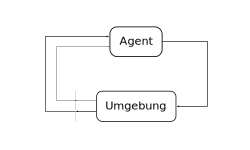
\includegraphics[keepaspectratio,width=0.75\textwidth]{abbildungen/schnittstelle_agent_umgebung.pdf}
  %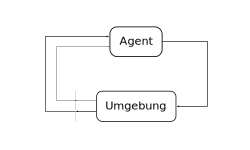
\includegraphics[height=0.5\textwidth, width=0.9\textwidth]{abbildungen/schnittstelle_agent_umgebung.pdf}
  \caption{Die Abbildung zeigt die Interaktion zwischen dem Agenten und der Umgebung, d.h. die Auswahl einer Aktion durch den Agenten basierend auf einem Zustand und die Reaktion der Umgebung in Form eines Rewards und eines Folgezustands.}
  \label{fig_schnittstelle}
\end{figure}

Das Ziel des Agenten beim Reinforcement Learning besteht darin, in jedem Zeitschritt seine Aktion so auszuwählen, dass die Gesamtmenge der vom ihm erhaltenen Belohnungen maximiert wird. Um dieses informelle Ziel zu formalisieren, wird der discounted Return $G_t$ zum Zeitpunkt $t$ definiert als

\begin{equation}
  G_t = R_{t+1} + \gamma R_{t+2} + \gamma R_{t+3} + \dotsb = \sum_{k=0}^{\infty} \gamma^k R_{t+k+1},
  \label{return_eq}
\end{equation}

wobei $\gamma \in [0, 1]$ als discount Faktor bezeichnet wird. Dieser regelt, wie stark zukünftige Rewards berücksichtigt werden. So ist ein Reward, der erst in $k$ Zeitschritten erhalten wird, um den Faktor $\gamma^{k-1}$ weniger Wert im Vergleich zu einem unmittelbar erhaltenen. Praktisch gesehen wird auf diese Art und Weise die Kurz- bzw. Weitsichtigkeit des Agenten reguliert. Im Falle episodischer Aufgaben vereinfacht sich die unendliche Summe aus Gleichung \eqref{return_eq} zu einer endlichen Summe. Dabei ist die obere Summationsgrenze $T$, d.h. der Zeitschritt des Terminalzustands $s_T$. Des Weiteren besitzt der Return die rekursive Eigenschaft $G_t = R_{t+1} + \gamma G_{t+1}$, welche für nachfolgende Definitionen von erheblicher Wichtigkeit ist.

Zum Erreichen seines Lernziels muss der Agent ein entsprechendes Verhalten erlernen, d.h. er muss für jeden Zustand $s_t$ die Aktion $a_t$ kennen, sodass schlussendlich die Summe der Belohnungen maximal wird. Zur Formalisierung des Verhaltens des Agenten, also der Auswahl von Aktionen unter Berücksichtigung des aktuellen Zustands, wird die sogenannte Policy $\pi: \mathcal{A} \times \mathcal{S} \to [0, 1]$ definiert. Dabei ist $\pi(s|a)$ eine Wahrscheinlichkeitsverteilung über alle möglichen Aktionen $a$ unter der Bedingung, dass sich die Umgebung im Zustand $s$ befindet. Zu Beginn des Lernprozesses wird die Policy für gewöhnlich zufällig initialisiert. Anschließend wird sie schrittweise solange verändert, bis keine Verbesserung mehr auftritt. Hat der Agent an diesem Punkt die ihm gestellte Aufgabe erfolgreich gelöst, ist dies in der Regel gleichbedeutend damit, dass er die optimale Policy oder eine Approximation selbiger erlernt hat. In der Zukunft kann er dann zur Bewältigung dieser Aufgabe einfach für jeden Zustand die Aktion mit der größten Wahrscheinlichkeit auswählen.

Um die Auswahl der aktuellen Aktion $a_t$ möglichst sinnvoll vorzunehmen, werden neben dem aktuellen Zustand $s_t$ auch Informationen darüber benötigt, inwiefern die aktuelle Entscheidung zukünftige Rewards beeinflusst. Nur so ist es dem Agenten möglich, die längerfristigen Folgen seines aktuellen Handelns abzuschätzen und somit die Summe über alle erhaltenen Rewards zu maximieren und nicht nur den Aktuellen. Der Agent würde also gerne wissen, \glqq wie gut \grqq{} es bezüglich zukünftiger Rewards ist, sich in einem bestimmen Zustand zu befinden bzw. eine bestimmte Aktion in einem bestimmten Zustand auszuführen. Zusammen mit der zuvor eingeführten Policy, die das zukünftige Verhalten des Agenten steuert, lassen sich entsprechende Bewertungsfunktionen definieren, die darüber Aufschluss geben. Hierzu wird eine State-Value Funktion wie folgend definiert:

\begin{equation*}
  v_\pi(s) = \mathbb{E}_\pi[G_t|s_t=s] = \mathbb{E}_\pi[\sum_{k=0}^{\infty} \gamma^k R_{t+k+1} | s_t=s], \quad \forall s \in \mathcal{S}
  \label{v_pi_eq}
\end{equation*}

Die State-Value Funktion eines Zustands $s$ für eine Policy $\pi$ entspricht dem erwarteten Return, der sich ergibt, wenn der Agent im Zustand $s$ startet und ab dort der Policy $\pi$ folgt, d.h. seine Aktionen basierend auf $\pi(a|s)$ auswählt. Dabei ist der Wert eines Terminalzustandes als Null definiert. Auch die State-Value Funktion verfügt über eine rekursive Eigenschaft, die widerum aus der des Returns resultiert. Die folgende Gleichung setzt den Wert des aktuellen Zustands $s$ in Beziehung zu den Werten möglicher Folgezustände $s'$ und wird als Bellmann-Gleichung für $v_\pi$ bezeichnet:

\begin{equation}
  v_\pi(s) = \mathbb{E}_\pi[R_{t+1} + \gamma G_{t+1} | s_t=s] = \sum_{a} \pi(a|s) \sum_{s'} p(s'|s,a) [r(s,a,s') + \gamma v_\pi(s')]
  \label{v_pi_bellmann_eq}
\end{equation}

Die Berechnung des Erwartungswertes kann sich dabei wie folgend vorgestellt werden. Zunächst werden die im Zustand $s$ möglichen Aktionen $a$ mit der auf der Policy $\pi(a|s)$ beruhenden Auftrittswahrscheinlichkeit gewichtet. Somit entstehen konkrete Auswahlen von $s$ und $a$. Hieraus wiederum resultieren Folgezustände $s'$, die ihrerseits mit der Zustands-Übergangs-Wahrscheinlichkeit $p(s'|s,a)$ gewichtet werden. Auf diese Art und Weise erhält jeder Summand, d.h. der Inhalt der Klammern für eine konkrete Wahl von $s$, $a$ und $s'$, seine eigene Gewichtung. Abschließend wird dann über alle entsprechend gewichtetet Möglichkeiten aufsummiert. Die Bellmann-Gleichung für $v_\pi$ bildet die theoretische Grundlage für viele Verfahren, die die State-Value Funktion erlernen. Im denkbar einfachsten Verfahren wird $v_\pi$ schrittweise berechnet, indem die rechte Seite von Gleichung \eqref{v_pi_bellmann_eq} als Update-Regel verwendet wird. Hierzu muss allerdings $p(s'|s,a)$ bekannt sein, was jedoch oftmals nicht der Fall ist.

Analog zu $v_\pi$ lässt sich die sogenannte Action-Value Funktion $q(s,a) = \mathbb{E}_\pi[G_t | s_t=s, a_t=a]$ definieren. Diese gibt den erwarteten Return an für den Fall, dass der Agent im Zustand $s$ die Aktion $a$ tätigt und ab da an der Policy $\pi$ folgt. Sie erlaubt somit eine Bewertung einer bestimmten Aktion in einem bestimmen Zustand unter Berücksichtigung einer Policy.

Da State-Value Funktionen die Möglichkeit bieten, eine Ordnung auf den Policys zu definieren, lässt sich eine optimale Policy auf die folgende Art und Weise definieren. Eine Policy $\pi$ ist besser oder gleich als eine policy $\pi'$, wenn der erwartete Return von $\pi$ für alle Zustände größer oder gleich ist als der von $\pi'$, d.h. $\pi \ge \pi'$, wenn $v_\pi(s) \ge v_{\pi'}$ für alle $s \in \mathcal{S}$. Es gibt immer mindestens eine Policy die besser als oder zumindest gleich ist im Vergleich zu allen anderen Policys. Dies ist die optimale Policy und sie wird mit $\pi_*$ bezeichnet. Die optimale State-Value Funktion $v_*$ wird definiert als $v_*(s) = max_\pi v_\pi(s)$ für alle $s \in \mathcal{S}$.

Ein Agent, dem es gelungen ist, die optimale Policy bzw. State-Value Funktion zu lernen, hat die ihm gestellte Aufgabe logischerweise im bestmöglichen Sinne gelöst. Leider tritt dieser Fall in der Realität so gut wie nie auf, sondern es sind in der Regel nur approximative Lösungen für die Policy bzw. State-Value Funktion möglich. Ursächlich hierfür sind hauptsächlich zwei Gründe. Zum einen ist die Zustands-Übergangs-Wahrscheinlichkeit $p(s'|s,a)$ oftmals nicht bekannt und zum anderen überschreitet der Rechenaufwand zur Bestimmung der optimalen Policy bzw. State-Value Funktion in der Regel die verfügbaren Ressourcen. So sind beispielsweise die Zustandsräume so groß, dass es aus Gründen der zur Verfügung stehenden Speichermenge unmöglich ist, für jeden Zustand $s$ den Wert von $v(s)$ vorzuhalten. In der Folge werden dann Funktionsapproximatoren wie beispielsweise Neuronale Netze für die eingesetzt, um die Policy und/oder die State-Value Funktion geeignet zu schätzen. Um die Parameter eines solchen Modells geeignet zu trainieren, wird ein entsprechender Lernalgorithmus benötigt. Dieser wird im nächsten Abschnitt präsentiert.


\section{Proximal Policy Optimization}
\label{sec_ppo}

Für die im weiteren Verlauf dieser Arbeit durchgeführten Experimente wird der \ac{PPO} Algorithmus verwendet. Dieser wurde von J. Schulman et. al. im Jahr 2017 veröffentlicht \cite{PPO}. Grundsätzlich handelt es sich bei \ac{PPO} um eine Policy Gradientenmethode und im Speziellen um ein sogenanntes Actor-Critic Verfahren. Policy Gradientenmethoden sind in der Lage eine parametrisierte Policy zu erlernen, wie sie im Rahem dieser Arbeit benutzt werden soll. Dazu wird ein skalares Leistungsmaß unter Berücksichtigung der Policy Parameter definiert, welches anschließend maximiert wird, indem ein Gradientenaufstieg durchgeführt wird. Actor-Critic Verfahren erweitern dieses Vorgehen. Die Policy, die die Auswahl der Aktionen vorgibt, wird als Actor bezeichnet. Der Critic bewertet die zuvor vom Actor ausgewählten Aktionen. Dazu erlernt er beispielsweise die State-Value Funktion. Auf Basis der Bewertung des Critics verbessert der Actor die Policy. Somit ist der grundlegende Ablauf von \ac{PPO} folgender. Durch eine Interaktion mit der Umgebung, d.h. basierend auf der Policy werden Aktionen ausgewählt und ausgeführt, werden Daten generiert. Diese werden anschließend genutzt, um unter Verwendung eines Gradientenaufstiegs die Verlustfunktion zu optimieren. Während herkömmliche Policy Gradientenmethoden nur ein Gradientenupdate pro Datenwert anwenden, haben Schulman et. al. in ihrem Paper eine neue Verlustfunktion präsentiert, die dazu geeignet ist, mehrere Trainingsepochen basierend auf denselben Daten durchzuführen. Hierdurch weißt \ac{PPO} eine erhöhte Effizienz bei der Nutzung der zum Training zur Verfügung stehenden Daten auf. Da sich gradientenbasierte Verfahren bei der Optimierung der Verlustfunktion sehr sensitiv hinsichtlich der Schrittweite verhalten, übernimmt \ac{PPO} diesbezüglich einige Vorteile des Trust Region Policy Optimization (TRPO) Algorithmus. Dieser benutzt eine Verlustfunktion, die sicherstellt, dass die nach einem Gradientenupdate erhaltene neue Policy nicht zu stark von der alten Policy abweicht und somit katastrophale Sprünge in der Performance der Policy verhindert. Allerdings erreicht TRPO dieses Ziel nur mit einem immensen Rechenaufwand, der sich entsprechend auch in einer erhöhten Komplexität bei der Implementierung niederschlägt. Dieses Problem überkommt \ac{PPO}, da er lediglich Ableitungen erster Ordnung verwendet. Des Weiteren ist \ac{PPO} sehr robust im Sinne, dass er sogut wie kein Hyperparameter-Tuning für verschiedene Lernprobleme benötigt. \\

Um die im Rahmen des \ac{PPO} Papers vorgestellte neue Verlustfunktion zu definieren, wird zunächst das Wahrscheinlichkeitsverhältnis $r_t(\theta) = \frac{\pi_\theta(a_t|s_t)}{\pi_{\theta_{old}}(a_t|s_t)}$ definiert, wobei $\pi_\theta$ die aktuelle Policy kennzeichnet und $\pi_{\theta_{old}}$ die Policy vor dem letzten Updateschritt. Somit ist $r_t(\theta)$ ein Maß dafür, wie stark sich die Wahrscheinlichkeit für die Auswahl der Aktion $a_t$ unter der Bedingung $s_t$ durch den letzten Updateschritt verändert hat. Wenn die Wahrscheinlichkeit größer geworden ist, dann ist $r_t(\theta) > 1$. Ist sie hingegen kleiner geworden, dann ist $0 < r_t(\theta) < 1$. Darüber hinaus gilt insbesondere $r(\theta_{old}) = 1$. Basierend auf $r_t(\theta)$ lässt sich eine Verlustfunktion $L^{CPI}(\theta) = \hat{\mathbb{E}}[r_t(\theta) \hat{A}_t]$ definieren. Hierbei steht CPI für conservative policy improvement und $\hat{a}_t$ ist eine Schätzung der Advantage Funktion zum Zeitpunkt $t$. Diese ist als $A(s,a) = Q(s,a) - V(s)$ definiert und gibt an wie viel besser bzw. schlechter es ist, die Aktion $a$ im Zustand $s$ auszuwählen. Die Maximierung von $L^{CPI}$ würde jedoch bei einem Updateschritt mitunter zu beliebig großen Veränderungen der Policy führen. Zur Lösung dieses Problems schlagen die Autoren folgende abgeschnittene Verlustfunktion vor:

\begin{equation}
  \label{L_CLIP}
	L^{CLIP} = \hat{\mathbb{E}}_t[min(r_t(\theta) \hat{A}_t, clip(r(\theta), 1-\epsilon, 1+\epsilon) \hat{A}_t)],
\end{equation}

wobei $\epsilon$ einen Hyperparameter beschreibt, der üblichweise aus dem Interval $[0.1, 0.2]$ stammt. Der erste Term innerhalb des Minimum-Operators ist die zuvor präsentierte Verlustfunktion $L^{CPI}$. Der zweite Term hingegen ist die abgeschnittene Variante selbiger. Der clip-Operator begrenzt den zulässigen Wertebereich von $r_t(\theta)$ auf das Interval $[1-\epsilon, 1+\epsilon]$, indem er $r_t(\theta)$ für Werte außerhalb dieses Intervals im Zweifelsfall abschneidet. Aus diesen beiden Termen wird abschließend das Minimum ausgewählt. Somit ist die Zielfunktion $L^{CLIP}$ eine untere Schranke für $L^{CPI}$. Mit dieser Methode wird eine zu große Veränderung des Wahrscheinlichkeitsverhältnisses ignoriert, wenn dadurch die Zielfunktion verbessert würde. Würde sie jedoch verschlechtert, so wird die entsprechende Veränderung inkludiert werden.

Das Verhalten der geclippten Zielfunktion \eqref{L_CLIP} wird durch Abbildung \ref{fig_L_clip} für einen einzelnen Zeitschritt $t$ verdeutlicht. Der rote Kreis entspricht dem Startpunkt der Optimierung, an dem $r = 1$ ist. Auf der linken Seite ist $L^{CLIP}$ für $A > 0$ dargestellt, d.h. die ausgeführte Aktion war besser als erwartet. Infolgedessen soll die Wahrscheinlichkeit, mit der die Aktion ausgewählt wird, erhöht werden. Um hierbei die Policy jedoch nicht zu stark zu verändern, wird $r$ bei $1+\epsilon$ geclipped. Der Fall $A < 0$ ist auf der rechten Seite abgebildet und in diesem war die ausgeführte Aktion schlechter als erwartet. Analog soll nun die dazugehörige Wahrscheinlichkeit verringert werden. Um wieder eine zu starke Veränderung der Policy zu verhindern, wird $r$ dieses mal bei $1-\epsilon$ geclipped. Die beiden zuvor angesprochenen Bereiche entsprechen dem Ignorieren einer zu großen Veränderung von $r$, wenn $L^{CLIP}$ dadurch verbessert würde. Das Inkludieren einer entsprechenden Veränderung, wenn dadurch die Zielfunktion verschlechtert würde, findet sich für $A < 0$ auf der ganz rechten Seite (und analog für $A > 0$ auf der ganz linken Seite). In diesem Fall wurde die Wahrscheinlichkeit für eine Aktion erhöht, obwohl diese schlechter als erwartet war. Somit wäre es wünschenswert, den letzten Gradientenschritt rückgängig zu machen und $L^{CLIP}$ ermöglich genau das. Die Funktion ist in diesem Bereich negativ, womit der Gradient in die entgegengesetzte Richtung zeigen wird und die Aktion im dem Maße, in dem sie zuvor wahrscheinlicher gemacht wurde, weniger wahrscheinlich machen wird.

\begin{figure}[ht!]
  \centering
  \includegraphics[height=0.5\textwidth, width=0.9\textwidth]{abbildungen/L_clip.pdf}
  \caption{Die Abbildung zeigt das Verhalten von $L^{CLIP}$ für einen einzelnen Zeitschritt $t$. Links ist der Fall $A > 0$ dargestellt, rechts der Fall $A < 0$.}
  \label{fig_L_clip}
\end{figure}

Zur Schätzung der Advantage Funktion kann eine abgeschnittene Form der Generalized Advantage Estimation verwendet werden. Diese Methode wurde von J. Schulman et. al. im Jahr 2016 publiziert \cite{GAE}. Sie bietet in gewisser Weise die Möglichkeit, die Varianz und den Bias des Schätzers zu regulieren. Dazu verwendet dieser die folgende Gleichung:

\begin{equation}
  \hat{A}_t = \delta_t + (\lambda \gamma) \delta_{t+1} + (\lambda \gamma)^2 \delta_{t+2} + \dots + (\lambda \gamma)^{T-t+1} \delta_{T-1} \qquad \text{mit } \delta_t = R_t + \gamma \hat{V}(s_{t+1}) - \hat{V}(s_t)
  \label{eq_gae}
\end{equation}

Dabei ist $\gamma$ wie gehabt der discount Faktor, $R_t$ der Reward im Zeitschritt t und $\hat{V}$ ist die geschätzte State-Value Funktion. Der Parameter $\lambda \in [0, 1]$ regelt das Verhältnis zwischen Bias und Varianz des Schätzers. Für die Randwerte von $\lambda$ ergeben sich folgende Spezialfälle. Für $\lambda = 0$ ergibt sich aus Gleichung \ref{eq_gae} die sogenannte Einschritt Temporal Difference, welche überlichweise einen Bias aufweist, allerdings keine Varianz. Für $\lamba = 1$ entspricht Gleichung \ref{eq_gae} der eines Monte Carlo Schätzers. Dieser weißt zwar keinen Bias auf, dafür aber eine hohe Varianz. Zusammenfassend ergibt sich, dass der Schätzer für $\lambda = 0$ varianzfrei ist und für $\lambda = 1$ biasfrei.

Viele Verfahren zur varianzreduzierten Schätzung der Advantage Funktion benutzen eine erlernte State-Value Funktion. Wenn darüber hinaus als Modell ein Neuronales Netzwerk verwendet werden soll, das geteilte Parameter für die Policy und die State-Value Funktion besitzt, muss die finale Verlustfunktion eine Kombination der zuvor präsentierten Verlustfunktion \eqref{L_CLIP} und eines auf der Value function basierenden Fehlers sein. Somit ergibt sich die folgende finale Verlustfunktion, die noch um einen Entropy-Bonus erweitert wurde, um eine ausreichende Exploration sicherzustellen:

\begin{equation}
	L_t^{CLIP+VF+S}(\theta) = \hat{\mathbb{E}}_t[L_t^{CLIP}(\theta) - c_1 L_t^{VF}(\theta) + c_2 S[\pi_\theta(s_t)]]
  \label{L_gesamt}
\end{equation}

Dabei sind $c_1$ und $c_2$ skalare Koeffizienten zur Gewichtung der einzelnen Terme. Der Term $L_t^{VF}$ ist die Verlustfunktion der geschätzten State-Value Funktion. Diese ist über den quadratischen Fehler $(V_\theta(s_t) - V_t^{targ})^2$ definiert.

Eine beispielhafte Implementierung eines \ac{PPO} Algorithmus, der Trajektorien fester Länge verwendet, wird nachstehend gezeigt. Dabei werden in jeder Iteration von jedem Actor zunächst über $T$ Zeitschritte Daten gesammelt, indem auf der Policy basierend Aktionen ausgeführt werden und die so entstehenden Trajektorien aufgezeichnet werden. Danach wird auf Basis dieser die Advantage Funktion geschätzt. Abschließend wird für alle zuvor gesammelten Daten die Verlustfunktion \eqref{L_gesamt} berechnet und optimiert, d.h. es wird es wird ein Gradientenschritt getätigt. Dazu werden die Daten in Minibatches der Größe $M<NT$ unterteilt, die wiederum für $K$ Epochen zum Training verwendet werden.

\begin{algorithm}
	\caption{\ac{PPO}, Actor-Critic Style}
	\begin{algorithmic}
		\For{$iteration=1,2,\dots$}
			\For{$actor=1,2,\dots,N$}
        \State Führe die Policy $\pi_{\theta_{old}}$ in der Umgebung für T Zeitschritte aus
				\State Berechne eine Schätung der Advantage function $\hat{A}_1,\dots,\hat{A}_T$
			\EndFor
			\State Optimiere $L^{CLIP+VF+S}$ bezüglich $\theta$ für $K$ Epochen und einer Minibatch Größe $M<NT$
			\State $\theta_{old} \gets \theta$
		\EndFor
	\end{algorithmic}
\end{algorithm}


\section{Neural Map}
\label{sec_neural_map}

Nachdem im vorangegangen Abschnitt mit dem \ac{PPO} Algorithmus eine Möglichkeit zum Trainieren einer entsprechend parametrisierten Policy gegeben wurde, soll im folgenden Abschnitt das im Rahmen dieser Arbeit hierfür verwendete Modell, die Neural Map, vorgestellt werden. Diese wurde von E. Parisotto und R. Salakhutdinov im Jahr 2018 veröffentlicht \cite{NeuralMap}. Es handelt sich bei der Neural Map um ein vollständig differenzierbares Modell zur Paremtrisierung einer Policy, das über einen externen Speicher mit trainierbarem Lese- und Schreiboperator verfügt.

Speicher bzw. ein Gedächtnis sind eine entscheidende Komponente, um einem Agenten sinnvolles Handeln zu ermöglichen. Ohne diese Komponente kann der Agent sein Verhalten nur durch seine aktuelle Wahrnehmung steuern und ist somit nicht in der Lage, längerfristige Pläne umzusetzen. Modelle, die externe Speicher verwenden, können im Wesentlichen in zwei Kategorien unterschieden werden, solche mit einem trainierbarem Schreiboperator und solche ohne einen. Zweitere haben für gewöhnlich eine feste Speichergröße. Ein solches Modell kann z.B. die letzten $N$ durch den Agenten beobachteten Zustände speichern. Da es aufgrund des nicht trainierbaren Schreiboperators nicht lernt, welche Informationen gespeichert werden sollen, lernt es, wie es auf den Speicher zugreifen muss. Dieser Ansatz besitzt jedoch zwei Nachteile. Zum einen kann der Speicher beliebig viele redundante Informationen enthalten. Zum anderen muss die Größe des Speichers geeignet gewählt werden, was in der Regel a priori Wissen über die Aufgabe des Agenten voraussetzt. Hat der Agent für seine aktuelle Aufgabe z.B. eine maximale Anzahl an Schritten vorgegeben, so sollte $N$ größer sein als diese. Modelle mit trainierbaren Schreiboperatoren sind potentiell leistungsfähiger, da sie erlernen können, welche Informationen sie speichern sollen und welche sie ignorieren. Sie benötigen somit kein a priori Wissen darüber, was sie speichern sollen und können Informationen für eine beliebige Zeitdauer speichern. Basierend auf dem zweiten Ansatz, d.h. einem Modell mit externem Speicher und trainierbarem Schreiboperator, entwickelten die Autoren die Neural Map, deren detailierte Struktur im Folgenden präsentiert wird.

Die Neural Map wurde für den Einsatzzweck entworfen, dass der Agent sich in einer 2- oder 3-dimensionalen Umgebung befindet. Während jeder Interaktion mit der Umgebung wird auf den internen Speicher zugegriffen in Form einer Leseoperation und einer anschließenden Schreiboperation. Dabei ist die Schreiboperation lokal beegrenzt, sodass nur die Stelle des internen Speichers beschrieben werden kann, die mit der aktuellen Position des Agenten in der Umgebung korrespondiert. Für die Einfachheit sei im Folgenden angenommen, dass sich der Agent in einer planaren Umgebung befindet, d.h. das sich seine Position in selbiger durch eine $x$- und eine $y$-Koordinate beschreiben lässt. Darüber hinaus wird angenommen, dass eine Koordinatentransformation $\psi(x,y)$ existiert. Diese bildet jede Postion $(x,y)$ des Agenten auf eine Speicherposition $(x',y')$ der Neural Map ab, wobei $x' \in \{0, \dots, W-1\}$ und $y' \in \{0, \dots, H-1\}$. Zur Vereinfachung der Notation seien im Folgenden alle Koordinaten durch $\psi$ in den Wertebereich zulässiger Speicherpositionen der Neural Map transformiert worden.

Der interne Speicher $M$ der Neural Map ist ein $C \times H \times W$ Feature Block. Dabei ist $C$ die Feature Dimension, $H$ ist die vertikale Größe und $W$ die horizontale Größe. Somit ist an jeder Position von $M$ ist ein $C$-dimensionales Feature gespeichert. Es ist $s_t$ der aktuelle Zustand, $M_t$ der aktuelle interne Speicher der Neural Map und $(x_t,y_t)$ die aktuelle Position des Agenten. Dann wird die Neural Map durch folgende Gleichungen beschrieben:

\begin{equation*}
  \begin{align*}
    r_t=read(M_t)&, \quad c_t=context(M_t, s_t, r_t), \\
    w_{t+1}^{(x_t,y_t)}=write(s_t, r_t, c_t, M_t^{(x_t,y_t)})&, \quad M_{t+1}=update(M_t, w_{t+1}^{(x_t,y_t)}), \\
    o_t=[r_t, c_t, w_{t+1}^{(x_t,y_t)}]&, \quad \pi_t(a|s)=\text{Softmax}(f(o_t))
  \end{align*}
\end{equation*}

Dabei ist $w_t^{(x_t,y_t)}$ das Feature an der Position $(x_t,y_t)$ zum Zeitpunkt $t$. Die Verkettung von Vektoren wird durch $[x_1, \dots, x_k]$ symbolisiert. Die Ausgabe der Neural Map zum Zeitpunkt $t$ durch durch $o_t$ gekennzeichnet. Diese wird anschließend von einem weiteren Neuronalen Netz $f$ verarbeitet, um die Policy $\pi(a|s)$ zu generieren. Die zuvor aufgestellten Gleichungen bzw. die damit korrespondierenden Operationen sollen nun ausführlicher erklärt werden.

\textbf{Global Read Operation:} Innerhalb der $read$ Operation durchläuft die aktuelle Neural Map $M_t$ ein Convolutional Neural Network, welches einen $C$-dimensionalen Feature-Vektor $r_t$ als Output generiert. Dieser Global Read Vektor $r_t$ kann als eine Zusammenfassung aller in der Neural Map gespeicherten Informationen angesehen werden. \\[0.1in]
\textbf{Context Read Operation:} Durch die $context$ Operation wird überprüft, ob gewisse Informationen bereits in der Neural Map vorhanden sind. Dazu werden zunächst der aktuelle Zustand $s_t$ und der aktuelle Global Read Vektor $r_t$ miteinander verkettet und mit einer Gewichtsmatrix $W$ multipliziert, um einen Query Vektor $q_t$ zu erhalten. Anschließend wird das Skalarprodukt des Query Vektors $q_t$ und jedes Feature Vektors der Neural Map M_t^{(x,y)} gebildet. Die auf diese Weise entstandenen Werte $a_t^{(x,y)}$ beschreiben die Ähnlichkeit der beiden zuvor miteinander verrechneten Vektoren. Als Nächstes werden diese Werte normalisiert, um eine Wahrscheinlichkeitsverteilung $\alpha_t^{(x,y)}$ über alle Positionen der Map zu generieren. Basierend auf dieser wird abschließend der gewichtete Durchschnitt aller Feature Vektoren $M_t^{(x,y)}$ berechnet, welcher im Weiteren auch als Context Read Vektor $c_t$ bezeichnet wird. Die zuvor beschriebenen Berechnungen lassen sich mit den folgenden Gleichungen zusammenfassen:
\begin{equation*}
  \begin{align*}
    q_t = W [s_t, r_t]&, \quad a_t^{x,y} = q_t \cdot M_t^{(x,y)}, \\
    \alpha_t^{(x,y)} = \frac{e^{a_t^{(x,y)}}}{\sum_{(w,z)} e^{a_t^{w,z}}}&, \quad c_t = \sum_{(x,y)} \alpha_t^{(x,y)} M_t^{(x,y)}
  \end{align*}
\end{equation*}
Die Context Read Operation ermöglicht es der Neural Map als eine Art assoziativer Speicher zu fungieren. Dazu übergibt der Agent einen mitunter unvollständigen Speicher, den Query Vektor $q_t$, an die Operation und diese gibt ihm den vervollständigten Speicher zurück, der widerum $q_t$ am ähnlichsten ist. Somit kann der Agent beispielsweise abfragen, ob er etwas zu seiner aktuellen Beobachtung Ähnliches bereits gesehen hat. \\[0.1in]
\textbf{Local Write Operation:} Die $write$ Operation generiert für die aktuelle Position des Agenten $(x_t,y_t)$ zum Zeitpunkt $t$ den $C$-dimensionalen Write Vektor $w_{t+1}^{(x_t,y_t)}$. Dazu erhält sie als Eingabe den aktuellen Zustand $s_t$, den aktuellen Global Read Vektor $r_t$, den aktuellen Context Read Vektor $c_t$ und den aktuellen Feature Vektor $M_t^{(x_t,y_t)}$ an der Position $(x_t.y_t)$. Diese Vektoren werden miteinander verkettet und anschließend von einem Neuronalen Netz $f_w$ verarbeitet, um den Write Vektor zu erzeugen, d.h. $w_{t+1}^{(x_t,y_t)} = f_w([s_t, r_t, c_t, M_t^{(x_t,y_t)}])$. Dieser Write Vektor fungiert als Schreibkandidat an der aktuellen Position $(x_t, y_t)$ \\[0.1in]
\textbf{GRU-based Local Write Operation:} Der zuvor beschriebene $write$ Operator generiert mit einem Neuronalen Netz den Write Vektor, mit welchem dann das Feature des internen Speichers an der entsprechenden Position einfach hart überschrieben wird. Alternativ zu diesem Vorgehen kann eine Schreiboperation verwendet werden, die von der sogenannten Gated Recurrent Unit inspiriert wurde. Diese berücksichtigt das zuvor an der entsprechenden Position gespeicherte Feature bei der Berechnung des neuen Write Vektors. Solche Schreiboperationen verfügen über eine lange Geschichte im Bereich rekurrenter Neuronaler Netze und haben in diesem Bereich ihre Fähigkeit zum Speichern von Informationen über einen langen Zeitraum schon oft unter Beweis gestellt. Die GRU-basierte Schreiboperation wird durch die folgenden Gleichungen definiert:

\begin{equation*}
  \begin{align*}
    r_{t+1}^{(x_t,y_t)} &= \sigma(W_r[s_t, r_t, c_t, M_t^{(x_t,y_t)}]) \\
    \hat{w}_{t+1}^{(x_t,y_t)} &= \tanh (W_{\hat{h}}[s_t, r_t, c_t] + U_{\hat{h}}(r_{t+1}^{(x_t,y_t)} \odot M_t^{(x_t,y_t)})) \\
    z_{t+1}^{(x_t,y_t)} & = \sigma(W_z[s_t, r_t, c_t, M_t^{(x_t,y_t)}]) \\
    w_{t+1}^{(x_t,y_t)} &= (1 - z_{t+1}^{(x_t,y_t)}) \odot M_t^{(x_t,y_t)} + z_{t+1}^{(x_t,y_t)} \odot \hat{w}_{t+1}^{(x_t,y_t)}
  \end{align*}
\end{equation*}
Dabei kennzeichnet $x \odot y$ das Hadamard-Produkt der Vektoren $x$ und $y$, d.h. die elementweise Multiplikation. Bei $W_*$ und $U_*$ handelt es sich um Gewichtsmatrizen. $\sigma(\cdot)$ ist die Sigmoidfunktion, die definiert ist als $\sigma(x) = \frac{1}{1+e^{-x}}$. In Anlehnung an die GRU-Terminologie wird $r_{t+1}^{(x_t,y_t)}$ als Reset Gate und $z_{t+1}^{(x_t,y_t)}$ als Update Gate bezeichnet. Diese beiden steuern, wie stark sich der neue Write Vektor $w_{t+1}^{(x_t,y_t)}$ von dem alten Feature an der entsprechenden Position des internen Speichers unterscheidet.\\[0.1in]
\textbf{Map Update Operation:} Für den nächsten Zeitschritt $t+1$ wird die dazugehörige Neural Map $M_{t+1}$ durch die $Update$ Operation erzeugt. Dabei ist die aktualisierte Neural Map $M_{t+1}$ bis auf an der Position des Agenten $(x_t,y_t)$ gleich der vorangegangenen Neural Map $M_t$. An dieser Position wurde der zuletzt generierte Write Vektor $w_{t+1}^{(x_t,y_t)}$ gespeichert, sodass sich die $Update$ Operation durch die folgende Gleichung beschreiben lässt:
\begin{equation*}
  \begin{align*}
    M_{t+1}^{(a,b)} =
    \begin{cases}
      w_{t+1}^{(x_t,y_t)}, & \quad \text{für} (a,b) = (x_t,y_t) \\
      M_t^{(a,b)}, & \quad \text{für} (a,b) \ne (x_t,y_t)
    \end{cases}
  \end{align*}
\end{equation*}

Die Abbildung \ref{fig_neural_map} gibt eine Übersicht über das Wechselspiel zwischen den einzelnen Operatoren und den daraus resultierenden Datenpfaden. Auf der linken Seite finden sich mit dem aktuellen Zustand des internen Speichers $M_t$ und dem aktuellen Zustand der Umgebung $s_t$ die Eingaben der Neural Map im Zeitschritt $t$. Anhand den von hier ausgehenden Pfeilen ist ersichtlich, in welche Operationen wiederum diese Als Eingabe eingehen. Entsprechendes gilt für die Ausgangspfeile auf der rechten Seite der jeweiligen Operatoren. Der gestrichtelte Pfeil deutet an, dass das Feature $M_t^{(x_t,y_t)}$ ein Teil des gesamten internen Speichers $M_t$ ist und somit aus diesem extrahiert werden kann. Verzweigungen der Datenpfade sind durch die schwarz ausgefüllten Kreise dargestellt. Auf der rechten Seite sind mit der Policy $\pi(a|s)$ und dem Folgezustand des internen Speichers $M_{t+1}$ die Ausgaben der Neural Map im Zeitschritt $t$ angegeben.


\begin{figure}[ht!]
  \centering
  \includegraphics[keepaspectratio,width=0.75\textwidth]{abbildungen/neural_map.pdf}
  %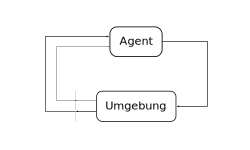
\includegraphics[height=0.5\textwidth, width=0.9\textwidth]{abbildungen/schnittstelle_agent_umgebung.pdf}
  \caption{Die Abbildung zeigt das Wechselspiel zwischen den verschiedenen Operatoren und die sich daraus ergebenen Datenpfade. Auf der linken Seite befinden sich mit $s_t$ und $M_t$ die Eingaben der Neural Map und auf der rechten Seite mit $\pi(a|s)$ und $M_{t+1}$ die Ausgaben. Die Wege dazwischen können anhand der Pfeile nachvollzogen werden.}
  \label{fig_neural_map}
\end{figure}


\section{Long short-term memory}
\label{sec_lstm}

Zum Abschluss dieses Kapitels wird eine kurze Einführung in das sogenannte Long Short-Term Memory (LSTM) gegeben. Es handelt sich bei dem LSTM um eine Architektur für ein rekurrentes Neuronales Netz, die von S. Hochreiter und J. Schmidhuber im Jahr 1997 publiziert wurde \cite{LSTM}. Im Jahr 1999 erhielt sie durch F. Gers et. al. noch eine entscheidende Erweiterung, wodurch der heute gebräuchliche Aufbau des LSTM entstand \cite{ForgetGate}. Besondere Anwendung findet das LSTM üblicherweise in der Analyse von Zeitreihen, es lässt sich aber auch zur Parametrisierung einer Policy im RL Kontext verwenden. Da es durch seine rekurrente Struktur in der Lage ist, Informationen über einen beliebigen Zeitraum zu speichern, dient das LSTM wie bereits im Neural Map Paper für die im Rahmen dieser Arbeit durchgeführten Experimente als Referenz.

Die entscheidende Komponente des LSTM zum Speichern von Informationen ist der Zellzustand $c_t$. Unter Verwendung mehrerer sogenannter Gates, namentlich des Forget Gates $f_t$, des Input Gates $i_t$ und des Output Gates $o_t$, wird der Datenfluss des Zellzustandes von einem zum nächsten Zeitschritt gesteuert. Jedes Gate erhält die Eingabe des LSTM $x_t$ und die vorherige Ausgabe des LSTM $h_{t-1}$ und berechnet daraus unter Verwendung eines Fully Connected Layers mit Sigmoid-Aktivierungsfunktion seine Ausgabe. Auf die gleiche Weise wird die Zellaktivierung $\hat{c}_t$ berechnet, allerdings wird hierbei $tanh$ als Aktivierungsfunktion verwendet. Der Zellzustand $c_t$ ergibt sich dann aus der Summe der Hadamard-Produkte von $f_t$ und $c_{t-1}$ und  $i_t$ und $\hat{c}_t$. Innerhalb dieser Summe reguliert das Forget Gate $f_t$, wie viel des vorherigen Zellzustandes $c_{t-1}$ vergessen bzw. übernommen wird. Über das Input Gate $i_t$ wird gesteuert, wie stark die aktuelle Zellaktivierung $\hat{c}_t$ berücksichtigt wird. Diese kann als Schreibkandidat für den Zellzustand angesehen werden. Anschließend kann die Ausgabe des LSTM $h_t$ berechnet werden aus dem Hadamard-Produkt von $o_t$ und dem Tangens hyperbolicus von $c_t$. Auf diese Weise bestimmt das Output Gate, in welchem Maße der Zellzustand in die Ausgabe des LSTM mit eingeht. Die zuvor beschriebene Struktur bzw. die Operationen können mit den folgenden Gleichungen zusammengefasst werden:

\begin{equation*}
\begin{align*}
	f_t &= \sigma(W_f x_t + U_f h_{t-1} + b_f) \\
	i_t &= \sigma(W_i x_t + U_i h_{t-1} + b_i) \\
	o_t &= \sigma(W_o x_t + U_o h_{t-1} + b_o) \\
	\hat{c}_t &= tanh(W_c x_t + U_c h_{t-1} + b_c) \\
	c_t &= f_t \odot c_{t-1} + i_t \odot \hat{c}_t \\
	h_t &= o_t \odot tanh(c_t)
\end{align*}
\end{equation*}

Dabei ist $\sigma(\dots)$ die Sigmoid-Funktion. Bei $W_*$ und $U_*$ handelt es sich um Gewichtsmatrizen und bei $b_*$ um Bias-Vektoren. Das Hadamard-Produkt zweier Vektoren wird durch $\odot$ gekennzeichnet.

\chapter{Experimente}

Dieses Kapitel beinhaltet die durchgeführten Experimente und die dazugehörigen Resultate. Für die Experimente werden eigens Umgebungen entworfen, um den Agenten mit spezifischen Problemstellungen zu konfrontieren. Dabei handelt es sich um zwei 2D-Umgebungen und eine 3D-Umgebung, in denen der Agent verschiedene Ziele suchen muss. Hierbei soll zum einen die Neural Map im Vergleich zum als Referenz gewählten LSTM betrachtet werden. Darüber hinaus soll ergründet werden, inwiefern die Erweiterung des Schreiboperators die Leistungsfähigkeit der Neural Map verbessert. Den Abschluss des Kapitels bildet eine Untersuchung der Neural Map als reine Speicherstruktur. Dabei wird selbige separiert auf ihre Fähigkeit untersucht, in ihrem internen Speicher eine Karte der Umgebung zu generieren.


\section{2D-Experimente}

Im folgenden Abschnitt wird das Verhalten der Neural Map in zwei eigens dafür konzipierten 2D-Umgebungen untersucht. Die Aufgabe innerhalb dieser Umgebungen besteht im Auffinden von Zielen in verschiedensten Konstellationen. Zunächst werden bis zu vier Ziele in einem hindernisfreien Raum gesucht. Anschließend werden bis zu drei Ziele in einem Labyrinth gesucht. Da in beiden Umgebungen die Ziele in einer bestimmten Reihenfolge aufgefunden werden müssen, kann es passieren, dass der Agent ein erst später zu erreichendes Ziel bereits zu einem früheren Zeitpunkt findet. Auf Basis dieses Ereignisses soll geklärt werden, inwiefern die Neural Map in der Lage ist, solche Ziele zu einem späteren Zeitpunkt möglichst effizient wiederzufinden. Dazu werden verschiedenen Varianten der Neural Map (mit/ohne Erweiterung des Schreiboperators) sowohl untereinander verglichen als auch mit einem LSTM.

Es sei an dieser Stelle noch auf folgenden Sachverhalt hingewiesen, der alle 2D-Experimente dieser Arbeit betrifft. Da der interne Speicher der Neural Map $M$ für alle Experimente in vertikaler und horizontaler Richtung die Größe $15$ aufweist und keine 2D-Umgebung größer als $15 \times 15$ ist, kann auf die in Abschnitt \ref{sec_neural_map} erwähnte Funktion $\psi$ zur Normalisierung der Koordinaten verzichtet werden. Stattdessen entspricht eine Position in der Umgebung exakt derselben Position im internen Speicher. Somit wird für kleinere Umgebungen nur ein entsprechender Teil von $M$ benutzt. Des Weiteren liefert die step-Methode aller Umgebungen nebem dem eigentlichen Zustand $s_t$ auch die aktuelle Position und Orientierung des Agenten. Diese werden jedoch niemals direkt an die Neural Map übergeben, sondern lediglich zum Bereitstellen der Eingabe $M_t^{(x_t,y_t)}$ sowie ggf. $M_t^{(x_{ext_t},y_{ext_t})}$ und für die Update Operation verwendet.

\subsection{Umgebung \glqq One\_Room\_Many\_Goals\_2D\grqq}

\begin{figure}[ht!]
  %\centering
  \begin{subfigure}[c]{0.45\textwidth}
    %\centering
    \includegraphics[keepaspectratio,width=\textwidth]{abbildungen/9x9_ep_start.pdf}
    \subcaption{}
    \label{fig_9x9_ep_start}
  \end{subfigure}
  \begin{subfigure}[c]{0.6\textwidth}
    %\centering
    \includegraphics[keepaspectratio,width=\textwidth]{abbildungen/9x9_sample_obs.pdf}
    \subcaption{}
    \label{fig_9x9_sample_obs}
  \end{subfigure}
  \caption{Die linke Abbildung (a) zeigt einen beispielhaften Episodenbeginn. Das rote Dreieck symbolisiert die Startposition und -orientierung des Agenten, das rote Rechteck die Beobachtung und die farbigen Kreise mit den Nummern die entsprechenden Ziele. Die rechte Abbildung (b) verdeutlicht die binäre Kodierung für die Kanäle 0 und 2 anhand einer beispielhaften Beobachtung.}
\end{figure}


Die Umgebung \glqq One\_Room\_Many\_Goals\_2D\grqq{} ist eine 2D-Umgebung und besteht aus einem Raum, d.h. einer rechteckigen hindernisfreien Fläche, die von einer durchgehenden Wand umgeben ist. In diesem Raum werden zu Beginn jeder Episode wahlweise $2$, $3$ oder $4$ Ziele platziert. Jedes Ziel hat eine eindeutige Nummer zwischen $1$ und $4$. Die Positionen der Ziele werden für jede Episode zufällig neu bestimmt. Dabei gelten folgende Regeln. Zwei aufeinander folgende Ziele dürfen nicht an derselben Position sein, d.h. Ziel 2 darf nicht auf Ziel 1 liegen, Ziel 3 nicht auf Ziel 2 und Ziel 4 nicht auf Ziel 3. Außerdem darf Ziel 1 nicht gleich mit der Startposition des Agenten sein. Der Agent wird zu Beginn jeder Episode auf einer fixen Startposition in der Mitte des Raumes positioniert. Die genauen Koordinaten der Startposition sind von der Größe des Raumes abhängig. Die initiale Blickrichtung des Agenten ist ebenfalls immer gleich, er guckt nach unten. Ein beispielhafter Episodenbeginn für einen Raum der Größe $9 \times 9$ mit 2 Zielen ist in Abbildung \ref{fig_9x9_ep_start} dargestellt. Das rote Dreieck markiert die Startposition und -orientierung des Agenten. Das rote Rechteck umfasst die Felder seiner initialen Beobachtung. Die farbigen Kreise mit den Nummern repräsentieren die beiden Ziele. Die Aufgabe des Agenten besteht dann darin, die Ziele in korrekter Reihenfolge abzulaufen, also zuerst Ziel 1, dann Ziel 2, usw. Hierfür erhält er in Abhängigkeit der Anzahl der Ziele eine entsprechende Belohnung für jedes Ziel. Dabei ist die Belohnung für das letzte Ziel immer signifikant größer als für die Zwischenziele. Auf diese Weise soll der Agent motiviert werden, alle Ziele zu erreichen. Zum Erledigen der Aufgabe steht dem Agenten eine maximale Anzahl an Schritten zur Verfügung. Diese ist abhängig von der Anzahl der Ziele und der Größe der Umgebung und wird stets so gewählt, dass der Agent nicht jedes Feld der Umgebung so oft ablaufen kann, wie es Zile gibt. Das Erreichen des Schrittlimits entspricht dem Übergang in einen Terminalzustand. Für diesen Terminalzustand sowie für jeden anderen getätigten Schritt erhält der Agent einen sogenannten Living-Reward von $-1 / Maximale\_Schrittanzahl$. Durch diesen und durch das Schrittlimit soll der Agent dazu animiert werden, die Aufgabe mit möglichst wenigen Schritten zu absolvieren. In Tabelle \ref{belohnung_ormg} ist der Zusammenhang zwischen der Größe der Umgebung, der Anzahl an Zielen, der Belohnungsstruktur und der maximalen Schrittanzahl übersichtlich zusammengefasst.

\begin{table}[h]
  \begin{tabular}{|>{\centering}m{2cm}|>{\centering}m{1.3cm}|>{\centering}m{1.8cm}|>{\centering}m{1.8cm}|>{\centering}m{1.8cm}|>{\centering}m{1.8cm}|>{\centering}m{2.3cm}|} \hline
    Größe der Umgebung & Anzahl Ziele & Belohnung Ziel 1 & Belohnung Ziel 2 & Belohnung Ziel 3 & Belohnung Ziel 4 & Maximale Schrittanzahl \tabularnewline \hline
    9x9 & 2 & 0.2 & 1.0 & - & - & 75 \tabularnewline \hline
    12x12 & 3 & 0.2 & 0.2 & 1.0 & - & 200 \tabularnewline \hline
    15x15 & 4 & 0.2 & 0.2 & 0.2 & 1.0 & 500 \tabularnewline \hline
  \end{tabular}
  \caption{Übersicht über die verschiedenen Größen der Umgebung \glqq One\_Romm\_Many\_Goals\_2D\grqq{} und die daraus resultierende Anzahl an Zielen, Belohnungsstruktur und maximale Schrittanzahl.}
  \label{belohnung_ormg}
\end{table}

Dem Agenten stehen in jedem Schritt drei mögliche Aktionen zur Verfügung: Gehe einen Schritt bzw. Feld nach vorne, also in Blickrichtung, oder drehe dich um $90\degree$ nach links oder rechts. Dabei kann der Agent nur freie Felder betreten, d.h. wenn der Agent vor sich eine Wand hat und trotzdem einen Schritt nach vorne macht, verändert sich seine Position nicht. Der Zustand $s_t$ ist ein Teilauschnitt der Umgebung in der Größe $(Anzahl\_Ziele + 1) \times 4 \times 3$. Das bedeutet, dass der Agent $4$ Felder geradeaus bzw. in Blickrichtung weit sehen. Zur Seite kann er jeweils 1 Feld sehen, sodass sich mit den Feldern links und rechts des Agenten sowie seinem eigenen die $3$ ergibt. Informationen über die Objekte der Umgebung, d.h. die Wände und die Ziele, sind in Analogie zum Neural Map Paper in den $(Anzahl\_Ziele + 1)$ binärkodierten Kanälen enthalten. Dabei enthält der nullte Kanal Informationen über die Lage der Wände. Hierbei entspricht eine $1$ einem Feld mit einer Wand und eine $0$ einem freien Feld. Die Kanäle $1$ bis $4$ spezifizieren die Positionen der entsprechenden Ziele. Dazu enthält der jeweilige Kanal genau eine $1$ an der Position des Ziels, alle anderen Einträge des Kanals sind $0$. In Abbildung \ref{fig_9x9_sample_obs} wird der Zusammenhang zwischem dem Teilauschnitt der Umgebung und dem daraus resultierenden binärkodierten Zustand $s_t$ für die Kanäle 0 und 2 beispielhaft verdeutlicht.

Folgende Überlegungen spielten beim Design der Umgebung eine Rolle. Zunächst wird durch die zufällige Positionierung der Ziele verhindert, dass es für den Agenten sinvoll ist, immer den gleichen Weg innerhalb der Umgebung zu wählen. Ihm bleibt nichts anderes übrig als, in jeder Episode aufs Neue den Raum zu erkunden. Bei dieser Erkundung kann es dann passieren, dass er Ziele sieht, die er erst zu einem späteren Zeitpunkt erreichen muss. Diese Situationen sind für die folgenden Untersuchungen von besonderem Interesse. Es wäre wünschenswert, wenn der Agent die Information über ein später zu erreichendes Ziel in seinem internen Speicher ablegen könnte und zu dem Zeitpunkt, wenn das entsprechende Ziel an der Reihe ist, wieder abrufen könnte. Basierend darauf sollte er im Idealfall dann einen möglichst direkten Weg zu dem entsprechenden Ziel wählen. Um die Wahrscheinlichkeit für solche Situationen zu erhöhen wird in den folgenden Experimenten sowohl die Anzahl der Ziele sukzessive erhöht, als auch die Größe der Umgebung. Durch die Vergrößerung der Umgebung benötigt der Agent mehr Schritte zur Erkundung selbiger, wobei mit jedem Schritt die Möglichkeit besteht, ein später zu erreichendes Ziel zu beobachten. Die Wahrscheinlichkeit dafür wird durch eine höhere Anzahl an Zielen noch zusätzlich erhöht. Außerdem kann auf diese Weise auch noch untersucht werden, wie gut der Agent mehrere zukünftige Ziele in der Neural Map abspeichern kann.

In den folgenden Experimenten werden vier verschiedene Varianten der Neural Map mit einem LSTM als Referenz verglichen. Die erste Variante der Neural Map entspricht der in Abschnitt \ref{sec_nm_impl} beschriebenen Implementierung. Durch die in Abschnitt \ref{sec_write_ext} eingeführte Erweitertung des Schreiboperators entsteht die zweite Variante. Die beiden weiteren Varianten entstehen dadurch, dass für den Schreiboperator und seine Erweiterung die in Abschnitt \ref{sec_neural_map} präsentierte GRU-based Local Write Operation verwendet wird. Die zum Training verwendeten Hyperparameter des PPO Algorithmus können der Tabelle \ref{hyperparam_ppo_ormg} entnommen werden. Diese sind für alle Experimente basierend auf der Umgebung \glqq One\_Room\_Many\_Goals\_2D\grqq{} und für alle zu untersuchenden Modelle gleich. Lediglich der Parameter $total\_timesteps$, der die für das Training zur Verfügung stehende Gesamtanzahl an Schritten spezifiziert, ist in Abhängigkeit der Umgebungsgröße und Anzahl an Zielen gewählt worden. Somit wird dieser auch in den entsprechenden Unterabschnitten angegeben. Im Anschluss an das Training wird das Modell für $10^5$ Zeitschritte in der jeweiligen Umgebung ausgeführt. Da angenommen wird, dass im internen Speicher der Neural Map $M_t$ eine Karte der Umgebung generiert wird, wird er beim Erreichen eines Terminalzustandes in seinen Initialzustand zurückgesetzt. In diesem enthält der Speicher in allen Einträgen Nullen. Dieses Zurücksetzen des Speichers wird sowohl im Training als auch in der Evaluation durchgeführt.

\begin{table}[h]
  \begin{center}
    \begin{tabular}{1 1}
      \hline
      nsteps & $512$ \\
      ent\_coef & $0.025$ \\
      lr & $0$ \\
      vf\_coef & $0$ \\
      max\_grad\_norm & $0$ \\
      gamma & $0.99$ \\
      noptepochs & $1$ \\
      cliprange & $0.0$ \\
      \hline
    \end{tabular}
  \end{center}
  \caption{Übersicht über die zum Training der Umgebung \glqq One\_Room\_Many\_Goals\_2D\grqq{} verwendeten Hyperparameter des PPO Algorithmus.}
  \label{hyperparam_ppo_ormg}
\end{table}


\subsubsection{Umgebungsgröße 9x9 und 2 Ziele}
Für das erste Experiment werden in einer Umgebung der Größe $9 \times 9$ zwei Ziele platziert. Die Abbildungen \ref{fig_9x9_ep_start} und \ref{fig_9x9_sample_obs} zeigen beispielhaft den Episodenbeginn und einen zufälligen Zeitschritt für die entsprechende Umgebungsgröße und Zielanzahl. Alle Modelle werden zunächst für $2,5\cdot10^6$ Zeitschritte trainiert und anschließend für $10^6$ ausgeführt zu Evaluationszwecken. Um die Leistungsfähigkeit der verschiedenen Modelle zu vergleichen, werden während der Evaluation sowohl die pro Episode erhaltenen Rewards als auch die Länge der Episoden aufgezeichnet. Durch die zufällige Platzierung der Ziele variiert auch die Anzahl benötigter Schritte pro Episode und infolgedessen auch der Reward pro Episode. Deshalb wird von diesen beiden Werten jeweils der Durchschnitt über alle erfolgreichen Episoden betrachtet. In Tabelle \ref{results9x9} sind die entsprechenden Ergebnisse aller Modelle zusammengefasst. Darüber hinaus enthält sie auch noch die Anzahl erfolgreich absolvierter Episoden. Hierbei fällt als Erstes auf, dass die Neural Map mit der Erweiterung des Schreiboperators (Neural Map + extW) die besten Ergebnisse erzielt. Sie absolviert in den $10^6$ zur Verfügung stehenden Zeitschritten 4338 erfolgreiche Episoden und benötigt im Durchschnitt für eine erfolgreich absolvierte Episode 21,73 Schritte. Dabei erreicht sie einen durchscnittlichen Reward von 0,91. Im Vergleich zur zweitbesten Variante (Neural Map + extW + GRU) benötigt sie somit ungefähr 2 Schritte weniger pro Episode. Die Grundvariante der Neural Map tätigt sogar ungefähr 3 Schritte mehr und die Referenz, das LSTM, ungefähr 5 Schritte. Die Verwendung der GRU-basierten Local Write Operation bringt hingegen keine Verbesserung und zwar sowohl bezüglich der Grundvariante der Neural Map als auch der Variante mit dem erweiterten Schreiboperator. Abschließend kann noch festgehalten werden, dass alle untersuchten Varianten der Neural Map bessere Ergebnisse erzielen als das LSTM.

\begin{table}[ht!]
  \begin{tabular}{|>{\centering}m{5cm}|>{\centering}m{2.2cm}|>{\centering}m{3.5cm}|>{\centering}m{3.5cm}|} \hline
    Modell  & Anzahl erfolgreicher Episoden & Durchschnittliche Schrittanzahl pro erfolgreicher Episode & Durchschnittlicher Reward pro erfolgreicher Episode \tabularnewline \hline
    LSTM & 3540 & 26,40 & 0,85 \tabularnewline \hline
    Neural Map & 3854 & 24,80 & 0,87 \tabularnewline \hline
    Neural Map + extW & \textbf{4338} & \textbf{21,73} & \textbf{0,91} \tabularnewline \hline
    Neural Map + GRU & 3717 & 25,12 & 0,86 \tabularnewline \hline
    Neural Map + extW + GRU & 4067 & 23,67 & 0,88 \tabularnewline \hline
  \end{tabular}
  \caption{Übersicht über die Anzahl erfolgreicher Episoden, deren durchschnittliche Länge und Reward für die Umgebung \glqq One\_Romm\_Many\_Goals\_2D\grqq{} in der Größe $9 \times 9$ mit 2 Zielen.}
  \label{results9x9}
\end{table}

Um einen detailiertern Einblick in das Verhalten der verschiedenen Modelle zu gewinnen, werden während der Evaluation nicht nur der Reward und die Schrittanzahl pro Episode aufgezeichnet, sondern auch die Observationen bzw. Zustände $s_t$, die Rewards $R_t$ und die Positionen des Agenten $(x_t,y_t)$. Hieraus lässt sich für jede Episode der gelaufene Weg des Agenten nachvollziehen. Darüber hinaus können mit diesen Daten die Positionen der Ziele rekonstruiert werden.

Da der Fokus des Experiments darauf liegt, inwiefern der Agent seinen internen Speicher zur Wegfindung nutzen kann, wird im folgenden der Weg vom ersten zum zweiten Ziel detailierter betrachtet. Dies geschieht aus den folgenden Gründen. Zu Beginn jeder Episode verfügt der Agent logischerweise über keinerlei Wissen bezüglich der Positionen der Ziele. Somit muss er den Raum jedes mal aufs Neue erkunden. Dabei wird er dann irgendwann zufällig auf sein erstes Ziel stoßen. Die dafür benötigte Anzahl von Schritten hängt jedoch in erster Linie von der zufälligen Position des Zieles ab und nicht vom Inhalt bzw. der Nutzung des internen Speichers. Dabei wird angenommen, dass der Agent die Umgebung möglichst effizient erkundet, d.h. gewisse Felder bzw. Bereiche werden nicht mehrfach betreten. Auch wenn der interne Speicher bei einer effizienten Erkundung durchaus von Nutzen sein kann, wird dies wird jedoch vernachlässigt. Somit ist der eigentliche Weg zum ersten Ziel von nachgeordnetem Interesse. Allerdings besteht die Möglichkeit, dass der Agent, während er auf der Suche nach dem ersten Ziel ist, das Zweite bereits sieht. Ist dies der Fall, so ist im Optimalfall der Weg vom ersten zum zweiten Ziel kein rein zufälliger Erkundungsweg mehr, sondern ein zielgerichtetes Wiederauffinden eines zuvor bereits beobachteten Ziels. Um den Weg des Agenten vom ersten zum zweiten Ziel zu bewerten, wird zunächst für jede Episode die optimale Anzahl an Aktionen ermittelt, die für diesen Weg benötigt wird. Diese ergibt sich in erster Linie aus dem Abstand der beiden Ziele, d.h. aus den Beträgen der Differenzen der x- und y-Koordinaten, und den dafür benötigten Schritten. Darüber hinaus werdem eventuell noch Drehungen benötigt. In Abhängigkeit der Orientierung des Agenten und der Lage der Ziele ergibt sich die Anzahl benötigter Drehungen entweder zu Null, Eins oder Zwei. Um auf aufwendige Fallunterscheidungen verzichten zu können, wird einfach immer von zwei Drehungen ausgegangen. Somit kann eine pessimistische Schätzung der optimalen Anzahl an Aktionen um von Ziel i zu Ziel j zu kommen mit der folgenden Formel berechnet werden:

\begin{equation}
  Optimale\_Schrittanzahl_{i,j} = |x_i - x_j| + |y_i - y_j| + 2
  \label{opt_steps_i_to_j}
\end{equation}

Von diesem Wert wird anschließend der Durchschnitt über alle Episoden gebildet. Ebenso wird für jede Episode die tatsächliche Anzahl benötigter Schritte für den entsprechenden Weg bestimmt, sowie der Durchschnitt über alle Episoden. Diese beiden Durchschnittswerte sowie deren Differenz, die der Anzahl zusätzlicher Schritte entspricht, sind für die betrachteten Modelle in Tabelle \ref{results9x9_1_to_2} zusammengefasst. Es zeigt sich, dass die durchschnittliche optimale Schrittanzahl für alle Modelle sehr ähnlich ist. Die Spannweite ist kleiner als 0,1 Schritte. Somit ist die durchschnittliche Entfernung zwischen den beiden Zielen in den betrachteten Episoden bei allen Modellen sehr ähnlich. Dies verleiht den Werten der tatsächlichen Schrittanzahl bzw. der Anzahl zusätzlicher Schritte mehr Aussagekraft, da diese wiederum immer in Bezug zur optimalen Schrittanzahl betrachtet werden müssen. So macht es einen erheblichen Unterschied, ob der Agent beispielsweise im Durchschnitt 5 zusätzliche Schritte tätigt bezogen auf einen optimalen Weg von 5 oder von 50 Schritten. Die Ergebnisse spiegeln die Gesamtlesitungen der verschiedenen Modelle aus Tabelle \ref{results9x9} wieder. Die Neural Map mit der Erweiterung des Schreiboperators benötigt im Durchschnitt die wenigsten zusätzlichen Schritte für den Weg von Ziel 1 zu Ziel 2. Darüber hinaus kommen alle Varianten der Neural Map mit weniger zusätzlichen Schritten aus als das LSTM.

\begin{table}[ht!]
  \begin{tabular}{|>{\centering}m{5cm}|>{\centering}m{2.9cm}|>{\centering}m{2.9cm}|>{\centering}m{3.3cm}|} \hline
    Modell  & Durchschnittliche optimale Schrittanzahl & Durchschnittliche tatsächliche Schrittanzahl & Durchschnittliche Anzahl zusätzlicher Schritte \tabularnewline \hline
    LSTM & 6,66 & 13,66 & 7,00 \tabularnewline \hline
    Neural Map & 6,75 & 13,11 & 6,36 \tabularnewline \hline
    Neural Map + extW & 6,71 & \textbf{12,40} & \textbf{5,69} \tabularnewline \hline
    Neural Map + GRU & 6,68 & 13,26 & 6,58 \tabularnewline \hline
    Neural Map + extW + GRU & 6,72 & 12,87 & 6,15 \tabularnewline \hline
  \end{tabular}
  \caption{Übersicht über die optimale Schrittanzahl, die tatsächliche Schrittanzahl und die Anzahl zusätzlicher Schritte bezogen auf den Weg von Ziel 1 zu Ziel 2 in der Umgebung \glqq One\_Romm\_Many\_Goals\_2D\grqq{} in der Größe $9 \times 9$ mit 2 Zielen.}
  \label{results9x9_1_to_2}
\end{table}

Anstatt den Durchschnitt über alle Episoden für den Weg vom ersten zum zweiten Ziel zu betrachten, werden die Episoden im folgenden in drei Mengen aufgeteilt. Alle Episoden, in denen bei der Suche nach dem ersten Ziel das zweite Ziel zu keinem Zeitpunkt gesichtet wurde, bilden die erste Menge. Diese Menge kann in gewisser Weise als Referenz für die beiden anderen Mengen betrachtet werden, da sich bei ihr die zufällige Suche für das zweite Ziel fortsetzt. Die zweite Menge enthält alle Episoden, in denen der Agent mindestens einmal über das zweite Ziel drüber gelaufen ist, d.h. das sich der Agent zu mindestens einem Zeitpunkt an exakt derselben Position wie Ziel 2 befunden hat. Hat der Agent das zweite Ziel lediglich gesichtet, ist jedoch nicht drüber gelaufen, so ist die entsprechende Episode Teil der dritten Menge. Für die drei Mengen werden die Bezeichnungen \glqq Ziel 2 nie beobachtet\grqq{}, \glqq Ziel 2 besucht\grqq{} und \glqq Ziel 2 gesehen\grqq{}. Für die Zuordnung der Episoden zu den jeweiligen Mengen werden alle zu einer Episode gehörenden Observationen betrachtet und hiervon wiederum speziell die mit dem zweiten Kanal bzw. Ziel korrespondierenden. Die Unterscheidung zwischen \glqq Ziel\grqq{} besucht und \glqq Ziel\grqq{} gesehen wird vorgenommen, da die Grundvariante der Neural Map nur die Speicherposition beschreibt, die der aktuellen Position des Agenten entspricht. Allerdings enthält die Observation des Agenten nicht nur Informationen über das Feld, auf dem er sich aktuell befindet, sondern auch noch über weitere Felder der Umgebung. Somit soll durch diese Unterscheidung untersucht werden, ob Informationen der Umgebung, die der aktuellen Position des Agenten entsprechen, anders verarbeitet werden beim Beschreiben des internen Speichers als die restlichen Informationen der Observation. Dazu wird für jede Episode wieder mit der Formel \ref{opt_steps_i_to_j} die optimale Schrittanzahl berechnet. Ebenso wird für jede Episode wieder die tatsächliche Schrittanzahl und die Anzahl zusätzlicher Schritte bestimmt. In Tabelle \ref{results9x9_1_to_2_per_M} sind die Durchschnittswerte der optimalen (Opt) und zusätzlichen Schrittanzahl (Differenz) für die verschiedenen Mengen für alle Modelle dargestellt. Dabei ist die Differenz zwischen optimaler und tatsächlicher Schrittanzahl einmal absolut (abs.) und einmal relativ (rel.) angegeben. Für die relative Differenz fungiert die optimale Schrittanzahl als Bezugsgröße, d.h. der absolute Wert durch diese dividiert und anschließend mit Hundert multipliziert für eine Angabe in Prozent. Bei den Ergebnissen fällt als Erstes auf, dass die optimale Schrittanzahl zwischen den Zielen für die jeweilige Menge relativ ähnlich ist. So liegt sie für die Menge \glqq Ziel 2 nie beobachtet\grqq{} zwischen 7,52 und 7,62, für die Menge \glqq Ziel 2 besucht\grqq{} zwischen 6,62 und 6,82 und für die Menge \glqq Ziel 2 gesehen\grqq{} zwischen 4,0 und 4,73. Darüber hinaus ist es auffällig, dass in den Episoden der Menge \glqq Ziel 2 gesehen\grqq{} die Ziele 1 und 2 wesentlich näher beieinander liegen als in den anderen beiden Mengen und alle Modelle in dieser Menge die geringste Anzahl zusätzlicher Schritte benötigen. Bezüglich der beiden Mengen \glqq Ziel 2 nie beobachtet\grqq{} und \glqq Ziel 2 besucht\grqq{} lässt sich bei den verschiedenen Modellen keine Systematik hinsichtlich der Anzahl zusätzlicher Schritte feststellen. Manche Modelle benötigen in der einen Menge weniger zusätzliche Schritte, manchen in der Anderen.

\begin{table}
  \begin{tabular}{|c|c|c|c|c|c|c|c|c|c|}
    \hline
    \multirow{3}{*}{Modell} & \multicolumn{3}{|c|}{Ziel 2 nie beobachtet} & \multicolumn{3}{|c|}{Ziel 2 besucht} & \multicolumn{3}{|c|}{Ziel 2 gesehen} \\ \cline{2-10}
    & \multirow{2}{*}{Opt} & \multicolumn{2}{|c|}{Differenz} & \multirow{2}{*}{Opt} & \multicolumn{2}{|c|}{Differenz} & \multirow{2}{*}{Opt} & \multicolumn{2}{|c|}{Differenz} \\ \cline{3-4} \cline{6-7} \cline{9-10}
    & & abs. & rel. & & abs. & rel. & & abs. & rel. \\ \hline
    LSTM & 7,52 & 9,61 & 128\% & 6,67 & 6,26 & 94\% & 4,42 & 3,03 & 69\% \\ \hline
    Neural Map & 7,53 & 6,65 & 88\% & 6,82 & 7,32 & 107\% & 4,00 & 1,44 & 36\% \\ \hline
    Neural Map + extW & 7,62 & 6,91 & 91\% & 6,78 & 5,69 & 84\% & 4,73 & 2,68 & 56\% \\ \hline
    Neural Map + GRU & 7,58 & 7,61 & 100\% & 6,65 & 7,01 & 105\% & 4,11 & 1,65 & 40\% \\ \hline
    Neural Map + extW + GRU & 7,60 & 7,16 & 94\% & 6,62 & 6,35 & 96\% & 4,64 & 2,75 & 59\% \\ \hline
  \end{tabular}
  \caption{Übersicht über die optimale (Opt) und zusätzliche Schrittanzahl (Differenz) für den Weg von Ziel 1 zu Ziel 2 aufgeteilt in die drei Mengen \glqq Ziel 2 nie beobachtet\grqq{}, \glqq Ziel 2 besucht\grqq{} und \glqq Ziel 2 gesehen\grqq{} für die Umgebung \glqq One\_Romm\_Many\_Goals\_2D\grqq{} in der Größe $9 \times 9$ mit 2 Zielen.}
  \label{results9x9_1_to_2_per_M}
\end{table}


\subsubsection{Umgebungsgröße 12x12 und 3 Ziele}

\begin{figure}[ht!]
  \centering
  \includegraphics[keepaspectratio,width=0.6\textwidth]{abbildungen/12x12_ep_start.pdf}
  %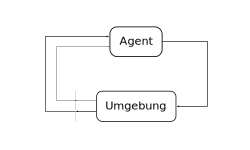
\includegraphics[height=0.5\textwidth, width=0.9\textwidth]{abbildungen/schnittstelle_agent_umgebung.pdf}
  \caption{Die Abbildung zeigt einen beispielhaften Episodenbeginn für die Umgebungsgröße $12 \times 12$ und 3 Ziele. Das rote Dreieck symbolisiert Startposition und -orientierung des Agenten, das rote Rechteck seine initiale Beobachtung und die farbigen Kreise mit den Nummern die entsprechenden Ziele. Die gestreichelten Pfeile zeigen einen möglichen optimalen Weg.}
  \label{fig_12x12_ep_start}
\end{figure}

Als nächstes wird die Größe der Umgebung auf $12 \times 12$ erhöht und es werden 3 Ziele in ihr platziert. Dadurch wird die Aufgabe für den Agenten anspruchsvoller. Ein beispielhafter Episodenbeginn ist in Abbildung \ref{fig_12x12_ep_start} dargestellt. Neben der Startposition des Agenten, seiner initialen Beobachtung und der Lage der Ziele ist ein möglicher optimaler Weg des Agenten durch die gestrichelten roten Pfeile angedeutet. Das beschreiten dieses Wegs ist jedoch höchst unwahrscheinlich, da der Agent hierfür die Lage der Ziele bereits kennen müsste. Dies ist jedoch selbstverständlich nicht der Fall. Der optimale Weg ist nur zur Veranschaulichung der Problemkomplexität eingezeichnet. In dieser Konfiguration werden alle Modelle für $5\cdot10^6$ Zeitschritte trainiert und anschließend wieder für $10^6$ Zeitschritte evaluiert. Die Auswertung entspricht im Wesentlichen der des vorangegangenen Abschnitts. Zunächst wird die Gesamtleistung der verschiedenen Modelle anhand der Anzahl erfolgreich absolvierter Episoden, der durchschnittlichen Länge und des durchschnittlichen Rewards pro erfolgreicher Episode beurteilt. Die entsprechenden Ergebnisse können der Tabelle \ref{results12x12} entnommen werden. Die beiden Varianten mit der Erweiterung des Schreiboperators erzielen bessere Ergebnisse als die beiden Variante ohne. Dabei erreicht die Variante der Neural Map mit der Erweiterung des Schreiboperators unter Verwendung des GRU-basierten Schreiboperators das beste Resultat mit durchschnittlich 84,08 Schritten pro erfolgreicher Episode. Insgesamt verbessert in dieser Konfiguration der Umgebung die Benutzung der GRU-basierten Schreiboperation die jeweilige Neural Map Variante. Des Weiteren liefern alle Varianten der Neural Map wieder bessere Ergebnis als das LSTM.

\begin{table}[ht!]
  \begin{tabular}{|>{\centering}m{5cm}|>{\centering}m{2.2cm}|>{\centering}m{3.5cm}|>{\centering}m{3.5cm}|} \hline
    Modell  & Anzahl erfolgreicher Episoden & Durchschnittliche Schrittanzahl pro erfolgreicher Episode & Durchschnittlicher Reward pro erfolgreicher Episode \tabularnewline \hline
    LSTM & 923 & 92,36 & 0,94 \tabularnewline \hline
    Neural Map & 975 & 88,53 & 0,96 \tabularnewline \hline
    Neural Map + extW & 995 & 86,73 & 0,97 \tabularnewline \hline
    Neural Map + GRU & 983 & 88,11 & 0,96 \tabularnewline \hline
    Neural Map + extW + GRU & \textbf{1053} & \textbf{84,08} & \textbf{0,98} \tabularnewline \hline
  \end{tabular}
  \caption{Übersicht über die Anzahl erfolgreicher Episoden, deren durchschnittliche Länge und Reward für die Umgebung \glqq One\_Romm\_Many\_Goals\_2D\grqq{} in der Größe $12 \times 12$ mit 3 Zielen.}
  \label{results12x12}
\end{table}

Mit der gleichen Begründung wie im vorherigen Abschnitt wird als nächstes wieder der Weg vom ersten zum zweiten Ziel detailierter untersucht. Dabei werden die Episoden wieder in die drei Mengen \glqq Ziel 2 nie beobachtet\grqq{}, \glqq Ziel 2 besucht\grqq{} und \glqq Ziel 2 gesehen\grqq{} aufgeteilt und es wird für jede Menge die durchschnittliche optimale Schrittanzahl und die durchschnittliche Anzahl zusätzlicher Schritte berechnet. Die entsprechenden Ergebnisse sind in Tabelle \ref{results12x12_1_to_2_per_M} dargestellt.

\begin{table}
  \begin{tabular}{|c|c|c|c|c|c|c|c|c|c|}
    \hline
    \multirow{3}{*}{Modell} & \multicolumn{3}{|c|}{Ziel 2 nie beobachtet} & \multicolumn{3}{|c|}{Ziel 2 besucht} & \multicolumn{3}{|c|}{Ziel 2 gesehen} \\ \cline{2-10}
    & \multirow{2}{*}{Opt} & \multicolumn{2}{|c|}{Differenz} & \multirow{2}{*}{Opt} & \multicolumn{2}{|c|}{Differenz} & \multirow{2}{*}{Opt} & \multicolumn{2}{|c|}{Differenz} \\ \cline{3-4} \cline{6-7} \cline{9-10}
    & & abs. & rel. & & abs. & rel. & & abs. & rel. \\ \hline
    LSTM & 9,17 & 23,31 & 254\% & 8,57 & 23,09 & 270\% & 4,40 & 11,62 & 264\% \\ \hline
    Neural Map & 8,35 & 26,07 & 312\% & 7,83 & 21,85 & 279\% & 4,08 & 5,63 & 138\% \\ \hline
    Neural Map + extW & 9,07 & 22,92 & 253\% & 8,19 & 22,73 & 277\% & 3,93 & 5,56 & 141\% \\ \hline
    Neural Map + GRU & 8,71 & 24,28 & 279\% & 8,28 & 22,21 & 268\% & 3,66 & 7,41 & 202\% \\ \hline
    Neural Map + extW + GRU & 9,13 & 23,87 & 261\% & 8,38 & 21,39 & 257\% & 4,5 & 9,34 & 208\% \\ \hline
  \end{tabular}
  \caption{Übersicht über die optimale (Opt) und zusätzliche Schrittanzahl (Differenz) für den Weg von Ziel 1 zu Ziel 2 aufgeteilt in die drei Mengen \glqq Ziel 2 nie beobachtet\grqq{}, \glqq Ziel 2 besucht\grqq{} und \glqq Ziel 2 gesehen\grqq{} für die Umgebung \glqq One\_Romm\_Many\_Goals\_2D\grqq{} in der Größe $12 \times 12$ mit 3 Zielen.}
  \label{results12x12_1_to_2_per_M}
\end{table}



\begin{table}
  \begin{tabular}{|c|c|c|c|c|c|c|c|c|c|}
    \hline
    \multirow{3}{*}{Modell} & \multicolumn{3}{|c|}{Ziel 2 nie beobachtet} & \multicolumn{3}{|c|}{Ziel 2 besucht} & \multicolumn{3}{|c|}{Ziel 2 gesehen} \\ \cline{2-10}
    & \multirow{2}{*}{Opt} & \multicolumn{2}{|c|}{Differenz} & \multirow{2}{*}{Opt} & \multicolumn{2}{|c|}{Differenz} & \multirow{2}{*}{Opt} & \multicolumn{2}{|c|}{Differenz} \\ \cline{3-4} \cline{6-7} \cline{9-10}
    & & abs. & rel. & & abs. & rel. & & abs. & rel. \\ \hline
    LSTM & 9,74 & 26,93 & 276\% & 8,69 & 21,64 & 249\% & 5,18 & 14,36 & 277\% \\ \hline
    Neural Map & 9,98 & 25,06 & 251\% & 8,21 & 21,68 & 264\% & 4,70 & 14,78 & 314\% \\ \hline
    Neural Map + extW & 9,59 & 24,29 & 253\% & 8,37 & 20,47 & 244\% & 5,51 & 14,12 & 256\% \\ \hline
    Neural Map + GRU & 9,83 & 29,57 & 301\% & 8,62 & 20,36 & 236\% & 5,85 & 8,68 & 148\% \\ \hline
    Neural Map + extW + GRU & 9,85 & 25,47 & 258\% & 8,34 & 17,22 & 207\% & 4,41 & 5,72 & 130\% \\ \hline
  \end{tabular}
  \caption{Übersicht über die optimale (Opt) und zusätzliche Schrittanzahl (Differenz) für den Weg von Ziel 2 zu Ziel 3 aufgeteilt in die drei Mengen \glqq Ziel 2 nie beobachtet\grqq{}, \glqq Ziel 2 besucht\grqq{} und \glqq Ziel 2 gesehen\grqq{} für die Umgebung \glqq One\_Romm\_Many\_Goals\_2D\grqq{} in der Größe $12 \times 12$ mit 3 Zielen.}
  \label{results12x12_2_to_3_per_M}
\end{table}



\subsubsection{Umgebungsgröße 15x15 und 4 Ziele}


\begin{figure}[ht!]
  \centering
  \includegraphics[keepaspectratio,width=0.6\textwidth]{abbildungen/15x15_ep_start.pdf}
  %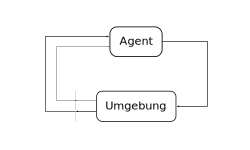
\includegraphics[height=0.5\textwidth, width=0.9\textwidth]{abbildungen/schnittstelle_agent_umgebung.pdf}
  \caption{Die Abbildung zeigt einen beispielhaften Episodenbeginn für die Umgebungsgröße $15 \times 15$ und 4 Ziele. Das rote Dreieck symbolisiert Startposition und -orientierung des Agenten, das rote Rechteck seine initiale Beobachtung und die farbigen Kreise mit den Nummern die entsprechenden Ziele. Die gestreichelten Pfeile zeigen einen möglichen optimalen Weg.}
  \label{fig_12x12_ep_start}
\end{figure}
total\_timesteps: $10\cdot10^6$

\begin{table}[ht!]
  \begin{tabular}{|>{\centering}m{5cm}|>{\centering}m{2.2cm}|>{\centering}m{3.5cm}|>{\centering}m{3.5cm}|} \hline
    Modell  & Anzahl erfolgreicher Episoden & Durchschnittliche Schrittanzahl pro erfolgreicher Episode & Durchschnittlicher Reward pro erfolgreicher Episode \tabularnewline \hline
    LSTM & 329 & 269,75 & 1,08 \tabularnewline \hline
    Neural Map & 365 & 242,12 & 1,12 \tabularnewline \hline
    Neural Map + extW & 397 & 230,25 & 1,14 \tabularnewline \hline
    Neural Map + GRU & 360 & 239,43 & 1,12 \tabularnewline \hline
    Neural Map + extW + GRU & \textbf{404} & \textbf{224,65} & \textbf{1,15} \tabularnewline \hline
  \end{tabular}
  \caption{Übersicht über die Anzahl erfolgreicher Episoden, deren durchschnittliche Länge und Reward für die Umgebung \glqq One\_Romm\_Many\_Goals\_2D\grqq{} in der Größe $15 \times 15$ mit 4 Zielen.}
  \label{results15x15}
\end{table}

\begin{table}
  \begin{tabular}{|c|c|c|c|c|c|c|c|c|c|}
    \hline
    \multirow{3}{*}{Modell} & \multicolumn{3}{|c|}{Ziel 2 nie beobachtet} & \multicolumn{3}{|c|}{Ziel 2 besucht} & \multicolumn{3}{|c|}{Ziel 2 gesehen} \\ \cline{2-10}
    & \multirow{2}{*}{Opt} & \multicolumn{2}{|c|}{Differenz} & \multirow{2}{*}{Opt} & \multicolumn{2}{|c|}{Differenz} & \multirow{2}{*}{Opt} & \multicolumn{2}{|c|}{Differenz} \\ \cline{3-4} \cline{6-7} \cline{9-10}
    & & abs. & rel. & & abs. & rel. & & abs. & rel. \\ \hline
    LSTM & 9,74 & 26,93 & 276\% & 8,69 & 21,64 & 249\% & 5,18 & 14,36 & 277\% \\ \hline
    Neural Map & 9,98 & 25,06 & 251\% & 8,21 & 21,68 & 264\% & 4,70 & 14,78 & 314\% \\ \hline
    Neural Map + extW & 9,59 & 24,29 & 253\% & 8,37 & 20,47 & 244\% & 5,51 & 14,12 & 256\% \\ \hline
    Neural Map + GRU & 9,83 & 29,57 & 301\% & 8,62 & 20,36 & 236\% & 5,85 & 8,68 & 148\% \\ \hline
    Neural Map + extW + GRU & 9,85 & 25,47 & 258\% & 8,34 & 17,22 & 207\% & 4,41 & 5,72 & 130\% \\ \hline
  \end{tabular}
  \caption{Übersicht über die optimale (Opt) und zusätzliche Schrittanzahl (Differenz) für den Weg von Ziel 1 zu Ziel 2 aufgeteilt in die drei Mengen \glqq Ziel 2 nie beobachtet\grqq{}, \glqq Ziel 2 besucht\grqq{} und \glqq Ziel 2 gesehen\grqq{} für die Umgebung \glqq One\_Romm\_Many\_Goals\_2D\grqq{} in der Größe $15 \times 15$ mit 4 Zielen.}
  \label{results15x15_2_to_3_per_M}
\end{table}

\begin{table}
  \begin{tabular}{|c|c|c|c|c|c|c|c|c|c|}
    \hline
    \multirow{3}{*}{Modell} & \multicolumn{3}{|c|}{Ziel 2 nie beobachtet} & \multicolumn{3}{|c|}{Ziel 2 besucht} & \multicolumn{3}{|c|}{Ziel 2 gesehen} \\ \cline{2-10}
    & \multirow{2}{*}{Opt} & \multicolumn{2}{|c|}{Differenz} & \multirow{2}{*}{Opt} & \multicolumn{2}{|c|}{Differenz} & \multirow{2}{*}{Opt} & \multicolumn{2}{|c|}{Differenz} \\ \cline{3-4} \cline{6-7} \cline{9-10}
    & & abs. & rel. & & abs. & rel. & & abs. & rel. \\ \hline
    LSTM & 9,74 & 26,93 & 276\% & 8,69 & 21,64 & 249\% & 5,18 & 14,36 & 277\% \\ \hline
    Neural Map & 9,98 & 25,06 & 251\% & 8,21 & 21,68 & 264\% & 4,70 & 14,78 & 314\% \\ \hline
    Neural Map + extW & 9,59 & 24,29 & 253\% & 8,37 & 20,47 & 244\% & 5,51 & 14,12 & 256\% \\ \hline
    Neural Map + GRU & 9,83 & 29,57 & 301\% & 8,62 & 20,36 & 236\% & 5,85 & 8,68 & 148\% \\ \hline
    Neural Map + extW + GRU & 9,85 & 25,47 & 258\% & 8,34 & 17,22 & 207\% & 4,41 & 5,72 & 130\% \\ \hline
  \end{tabular}
  \caption{Übersicht über die optimale (Opt) und zusätzliche Schrittanzahl (Differenz) für den Weg von Ziel 2 zu Ziel 3 aufgeteilt in die drei Mengen \glqq Ziel 2 nie beobachtet\grqq{}, \glqq Ziel 2 besucht\grqq{} und \glqq Ziel 2 gesehen\grqq{} für die Umgebung \glqq One\_Romm\_Many\_Goals\_2D\grqq{} in der Größe $15 \times 15$ mit 4 Zielen.}
  \label{results15x15_2_to_3_per_M}
\end{table}

\begin{table}
  \begin{tabular}{|c|c|c|c|c|c|c|c|c|c|}
    \hline
    \multirow{3}{*}{Modell} & \multicolumn{3}{|c|}{Ziel 2 nie beobachtet} & \multicolumn{3}{|c|}{Ziel 2 besucht} & \multicolumn{3}{|c|}{Ziel 2 gesehen} \\ \cline{2-10}
    & \multirow{2}{*}{Opt} & \multicolumn{2}{|c|}{Differenz} & \multirow{2}{*}{Opt} & \multicolumn{2}{|c|}{Differenz} & \multirow{2}{*}{Opt} & \multicolumn{2}{|c|}{Differenz} \\ \cline{3-4} \cline{6-7} \cline{9-10}
    & & abs. & rel. & & abs. & rel. & & abs. & rel. \\ \hline
    LSTM & 9,74 & 26,93 & 276\% & 8,69 & 21,64 & 249\% & 5,18 & 14,36 & 277\% \\ \hline
    Neural Map & 9,98 & 25,06 & 251\% & 8,21 & 21,68 & 264\% & 4,70 & 14,78 & 314\% \\ \hline
    Neural Map + extW & 9,59 & 24,29 & 253\% & 8,37 & 20,47 & 244\% & 5,51 & 14,12 & 256\% \\ \hline
    Neural Map + GRU & 9,83 & 29,57 & 301\% & 8,62 & 20,36 & 236\% & 5,85 & 8,68 & 148\% \\ \hline
    Neural Map + extW + GRU & 9,85 & 25,47 & 258\% & 8,34 & 17,22 & 207\% & 4,41 & 5,72 & 130\% \\ \hline
  \end{tabular}
  \caption{Übersicht über die optimale (Opt) und zusätzliche Schrittanzahl (Differenz) für den Weg von Ziel 3 zu Ziel 4 aufgeteilt in die drei Mengen \glqq Ziel 2 nie beobachtet\grqq{}, \glqq Ziel 2 besucht\grqq{} und \glqq Ziel 2 gesehen\grqq{} für die Umgebung \glqq One\_Romm\_Many\_Goals\_2D\grqq{} in der Größe $15 \times 15$ mit 4 Zielen.}
  \label{results15x15_3_to_4_per_M}
\end{table}

\subsection{Four\_Ways\_Many\_Goals\_2D}


\begin{figure}[ht!]
  \centering
  \includegraphics[keepaspectratio,width=0.5\textwidth]{abbildungen/fwmg.pdf}
  %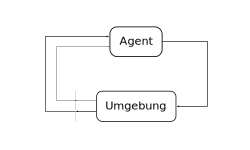
\includegraphics[height=0.5\textwidth, width=0.9\textwidth]{abbildungen/schnittstelle_agent_umgebung.pdf}
  \caption{Die Abbildung zeigt das Labyrinth der Umgebung \glqq Four\_Ways\_Many\_Goals\grqq{}. Der Agent startet zu Beginn jeder Episode auf dem zentralen Feld (rotes Dreieck) und erhält als Beobachtung einen Ausschnitt dem roten Rechteck entsprechend. Die grünen Kreise mit dem Buchstaben Z symbolisieren die möglichen Positionen zur Platzierung der Ziele.}
  \label{fig_fwmg_ep_start}
\end{figure}

Die Umgebung \glqq Four\_Ways\_Many\_Goals\_2D \grqq{} ist eine 2D-Umgebung im Stile eines Labyrinths. Sie verfügt über eine fixe Größe von 9 Feldern in horizontaler Richtung und 9 Feldern in vertikaler Richtung. Vom zentralen Punkt der Umgebung geht in jede der vier Richtungen ein Weg aus. Dieser Weg verzweigt sich dann ggf. noch ein weiteres mal. Auf jedem Weg gibt es eine Position zur Platzierung eines Ziels. Zu Beginn einer Episode werden auf diesen vier Position zwischen zwei und vier Ziele zufällig positioniert.

Diese Ziele verfügen wieder über eine eindeutige Nummer. Der Agent beginnt jede Episode auf dem zentralen Feld in der Mitte und startet für jede Episode neu bestimmten zufälligen Blickrichtung. Die Aufgabe des Agenten besteht wieder darin, die Ziele in der korrekten Reihenfolge abzulaufen. Die dafür verwendete Struktur der Rewards entsprecht der aus der vorherigen Umgebung. Lediglich die maximale Schrittanzahl unterscheidet sich. Für zwei Ziele stehen dem Agenten maximal XXX Schritte zur Verfügung, für drei Ziele YYY Schritte und für vier Ziele ZZZ Ziele.

Der Zustand $s_t$ ist hinsichtlich der binärkodierten Kanäle genau so aufgebaut wie bei der vorherigen Umgebung. Lediglich die Sichtreichweite in Blickrichtung wird um ein Feld reduziert, um der vermeintlich kleinen Umgebung genüge zu tragen. Somit ergibt sich die Größe des Zustands $s_t$ zu $(Anzahl_Ziele + 1) \times 3 \times 3$.

Bei dieser Umgebung wird der Agent im Vergleich zur vorherigen Umgebung zusätzlich mit Hindernissen konfrontiert.


\section{3D-Experiment}

Nachdem zuvor das Verhalten der Neural Map in verschiedenen 2D-Umgebungen ausführlich untersucht wurde, soll nun eine 3D-Umgebung verwendet werden.

Die 3D-Umgebung wird auf Basis von ViZDoom erstellt. ViZDoom basiert auf dem Computerspiel Doom und ermöglicht es, selbiges im RL Kontext zu benutzen.

Die Umgebung ist eine Adaption der 2D-Umgebung \glqq One\_Room\_Many\_Goals\grqq{}. Sie besteht somit aus einem quadratischem Raum. In diesem Raum werden zufällig zwei Ziele platziert, eine grüne Säule und eine rote Säule. Für die Platzierung der Ziele stehen insgesamt XXX mögliche Positionen zur Verfügung, wobei diese auf die beiden Raumhälften aufgeteilt sind. Zunächst wird zufällig eine dieser Positionen für das grüne Ziel ausgewählt. Um zu verhindern, dass die beiden Ziele zu nah beieinander liegen, stehen für die anschließende Platzierung des roten Ziels nur die Positionen in der anderen Raumhälfte zur Verfügung. Der Agent startet immer auf einer fixen Position in der Mitte des Raumes, die initiale Blickrichtung ist ebenfalls immer dieselbe. Die Aufgabe des Agenten ist es, zuerst zum grünen Säule und dann zur roten Säule zu laufen. Hierfür erhält er für das Erreichen der grünen Säule einen Reward von 0,2 und für das Erreichen der roten Säule einen Reward von 1,0. Dafür stehen dem Agenten XXX Schritte zur Verfügung. Für jeden Schritt erhält er wieder einen Living-Reward von $-1/Maximale\_Schrittanzahl.

Der Agent kann zwischen den drei Aktionen \glqq Drehung links\grqq{}, \glqqDrehung rechts\grqq{} und \glqq Gehe geradeaus\grqq{} auswählen. Dazu erhält er als Observation ein RGB-Array der Dimensionalität $120 \times 160 \times 3$.



\section{Untersuchung der Neural Map als reine Speicherstruktur}

Im folgenden Experiment soll die Neural Map außerhalb des bisherigen RL Kontexts untersucht werden. Es soll herausgefunden werden, inwiefern sich die Neural Map als reine Speicherstruktur nutzen lässt. Hierbei ist insbesondere von Interesse, inwiefern die Neural Map in ihrem internen Speicher eine Karte der Umgebung generieren kann. Um dies zu ergründen, wird eine leicht abgeänderte Form der Neural Map im Supervised Lernkontext betrachtet. Dazu werden folgende Annahmen getätigt. Zunächst wird wie in den 2D-Experimenten die vertikale und horizontale Größe des internen Speichers entsprechend der Umgebungsgröße gewählt. Somit entspricht eine Position in der Umgebung exakt einer Speicherposition. Die Informationen über die Umgebung, d.h. das Vorhandensein von Wänden bzw. freien Feldern und die Lage der Ziele, sind wie in den Abschnitten XXX und YYY beschrieben binär kodiert. Daraus ergibt sich, dass für jede Position der Umgebung ein entsprechend binärkodierter Umgebungsvektor existiert. Da es zu jeder Position in der Umgebung genau eine Position im internen Speicher gibt und sich das Feature an dieser Speicherposition nur durch seine Dimensionalität von dem Umgebungsvektor unterscheidet, wird das Feature als kodierte Form des Umgebungsvektors angesehen. Dabei ist die Kodierung zunächst unbekannt. Auf Basis dieser Annahmen wird für das Experiment eine leicht modifizierte Variante der Neural Map erstellt. Diese erhält als Eingabe wie gehabt eine Observation $s_t$ und den aktuellen Inhalt des internen Speichers $M_t$ und schätzt auf Basis dieser den Umgebungsvektor an der entsprechenden Position $(x_t, y_t)$. Im Fall der Neural Map mit der Erweiterung des Schreibvektors wird zusätzlich auch noch der Umgebungsvektor an der Position $(x_{ext_t},y_{ext_t})$ geschätzt. Im Folgenden wird wegen der besseren Lesbarkeit darauf verzichtet, immer darauf hinzuweisen, dass in Abhängigkeit der Benutzung des erweiterten Schreiboperators wahlweise ein oder zwei Vektoren von der modifizierten Variante der Neural Map geschätzt bzw. erzeugt werden.

Die für die Experimente benötigten Daten bilden Paare der Form (Eingabe, wahre Ausgabe). Um diese zu generieren, wird den 2D-Umgebungen eine zusätzliche Methode hinzugefügt. Diese erzeugt eine zufällige Observation aus der entsprechenden Umgebung. Dazu wird zunächst zufällig eine gültige Position des Agenten bestimmt, d.h. eine Position auf einem freien Feld. Anschließend wird auch die Orientierung zufällig gewählt und die zu der Positon und Orientierung gehörige Observation zurückgegeben. Da im Supervised Kontext auch die wahre Ausgabe bekannt sein muss, wird eine weitere Methode benötigt. Diese gibt die gesamte Umgebung zurück, d.h. die Umgebungsvektoren für alle Positionen, und wird einmal zu Beginn des Experiments aufgerufen. Im weiteren Verlauf können dann hieraus die jeweils benötigten Umgebungsvektoren auf Basis der Positionen extrahiert werden. Auf diese Weise werden die benötigten paarweisen Datenpunkte generiert.

Da die Neural Map nun als Ausgabe auch einen Vektor mit der gleichen Dimensionalität wie der Umgebungsvektor erzeugen muss, wird sie entsprechend modifiziert. Dazu wird zunächst das finale Neuronale Netz der Neural Map entfernt, da dessen Zweck in der Schätzung der Policy liegt und diese in diesem Experiment nicht benötigt wird. Das so veränderte Modell erzeugt als Ausgabe den Schreibvektor $w_{t+1}^{(x_t,y_t)}$ mittels der Local Write Operation. Da dieser noch über eine andere Dimensionalität als der Umgebungsvektor verfügt, wird er anschließend von einer weiteren Fully-Connected Schicht verarbeitet. Diese kann als Dekoder angesehen werden, da sie zur Schätzung des Umgebungsvektors das entsprechend kodierte Feature dekodiert. Somit generiert die entsprechend abgeänderte Neural Map als Ausgabe einen Vektor in der gleichen Dimensionalität wie der Umgebungsvektor. Damit die Einträge des geschätzten Umgebungsvektors auch aus dem Intervall $[0, 1]$ kommen, wird als Aktivierungsfunktion in der Dekoder-Schicht die Sigmoid-Funktion verwendet.

Nun kann wie im Supervised Kontext üblich die Ausgabe des Modells, also die Schätzung, mit der wahren Ausgabe verglichen werden, indem die Differenz der beiden Vektoren gebildet wird. Auf diesen Differenzvektor wird dann der mittlere quadratische Fehler angewendet. Die so entstehende Verlustfunktion kann nun mit einem entsprechenden Optimierer minimiert werden. Dazu berechnet selbiger den Gradienten des Modells und ändert auf Basis dessen die Parameter des Modells. Hierzu wird der sogenannte Adam Optimierer verwendet. Seine Parameter entsprechen den Standardwerten und als Lernrate wird $3e-4$ verwendet. Die Modelle werden jeweils für $25.000$ Schritte trainiert.

Für die Experimente wird zum einen die Umgebung \glqq One\_Room\_Many\_Goals\grqq{} in der Größe $9 \times 9$ mit 4 Zielen verwendet und die Umgebung \glqq Four\_Ways\_Many\_Goals\grqq{} ebenfalls mit 4 Zielen. Als Modelle werden die Grundvariante der Neural Map und die Variante mit der Erweiterung des Schreiboperators betrachtet. Von jeder der beiden Umgebungen werden 10 zufällige Konfigurationen verwendet, auf Basis derer die beiden Modelle trainiert werden. Eine Konfiguration entspricht dabei einer bestimmten Platzierung der 4 Ziele und wird paarweise für beide Modelle verwendet, um die entsprechenden Ergebnisse vergleichen zu können. Lediglich die zum Training verwendeten zufälligen Observationen unterscheiden sich noch. Nach dem Ende des Traingsprozesses wird abschließend die Güte der erzeugten Karte bewertet, indem für alle gültigen Position bzw. freien Felder die Differenz zwischen den geschätzten und tatsächlichen Umgebungsvektoren bestimmt wird und auf diesen anschließend der Mean-Squared-Error berechnet wird.

Die Abbildungen \ref{fig_mem_test_ormg} und \ref{fig_mem_test_fwmg} zeigen beispielhafte Verläufe des Mean-Squared-Errors über die Anzahl der Trainingschritte für die jeweiligen Umgebungen. Dabei ist auffällig, dass der MSE zu Beginn des Trainings relativ schnell bis ungefähr $0,2$ abfällt, ehe er dann für eine längere Zeit auf diesem Wert verweilt, bevor er wiederum weiter abfällt und seinen Endwert erreicht. In allen betrachteten Konfigurationen liegt der MSE am Ende des Trainings in der Größenordnung zwischen $10^-4$ und $10^-5$. Diese Werte werden auch bei der zuvor beschriebenen abschließenden Güteberechnung der Karte erreicht. Auch bei einer Sichtung der erzeugten Karten durch das menschliche Auge konnten die Positionen der Ziele fehlerfrei identifiziert werden, d.h. die entsprechende Eins in dem Umgebungsvektor war hinreichend signifikant.


\begin{figure}[ht!]
  \centering
  %\includegraphics[keepaspectratio,width=1.0\textwidth]{abbildungen/mem_test_ormg.pdf}
  \includegraphics[height=0.575\textwidth, width=0.9\textwidth]{abbildungen/mem_test_ormg.pdf}
  \caption{Die Abbildung zeigt die Entwicklung des Mean-Squared-Error über die Anzahl der Trainingschritte für die Neural Map und die Neural Map mit der Erweiterung des Schreiboperators für die Umgebung \glqq One\_Room\_Many\_Goals\grqq{}.}
  \label{fig_mem_test_ormg}
\end{figure}

\begin{figure}[ht!]
  \centering
  %\includegraphics[keepaspectratio,width=1.0\textwidth]{abbildungen/mem_test_fwmg.pdf}
  \includegraphics[height=0.575\textwidth, width=0.9\textwidth]{abbildungen/mem_test_fwmg.pdf}
  \caption{Die Abbildung zeigt die Entwicklung des Mean-Squared-Error über die Anzahl der Trainingschritte für die Neural Map und die Neural Map mit der Erweiterung des Schreiboperators für die Umgebung \glqq Four\_Ways\_Many\_Goals\grqq{}.}
  \label{fig_mem_test_fwmg}
\end{figure}

\chapter{Fazit und Ausblick}

Im Rahmen dieser Arbeit wurde eine Erweiterung für den Schreiboperators der Neural Map präsentiert.


%%% Literaturverzeichnis
\bibliographystyle{unsrtdin}	% eventuell durch andere Vorlage ersetzen
\bibliography{bibtex/literatur}


%%% Anhang
\cleardoublepage
\appendix
\renewcommand{\theequation}{\Alph{chapter}.\arabic{equation}}
\renewcommand{\thetable}{\Alph{chapter}.\arabic{table}}
\renewcommand{\thefigure}{\Alph{chapter}.\arabic{figure}}
\setcounter{equation}{0}
\setcounter{table}{0}

%\include{anhang/abbildungen}
\addappheadtotoc

%\addchap{Abkürzungsverzeichnis}
\chapter{Abkürzungsverzeichnis}
\begin{acronym}
 \acro{PPO}{Proximal Policy Optimization}
\end{acronym}



%%% Eidesstattliche Versicherung
%%\null
%%\thispagestyle{plain}
\cleardoublepage
%\addcontentsline{toc}{chapter}{Eidesstattliche Versicherung}

% Erst zum Ende einkommentieren, sonst gibts Probleme beim externalisieren von TiKz Graphiken.
%\includepdf[pages=1,scale=0.9,pagecommand={\thispagestyle{plain}}]{anhang/Eidesstattliche_Versicherung.pdf}


\end{document}
